\documentclass{article}                            %for shorter notes
\usepackage{graphics}                              %for EPS images (latex)
\usepackage{color}                                 %for defining custom colors
\usepackage{framed}                                %for shaded and framed paragraphs
\usepackage{textcomp}                              %for various symbols, e.g. Registered Mark
\usepackage{geometry}                              %for defining page size
\usepackage{longtable}                             %for breaking tables
\usepackage{listings}                              %for code listings
\usepackage[linkbordercolor={1.0 1.0 0.0}]{hyperref} %for \url tag
\lstloadlanguages{bash,XML}
\usepackage{multirow}
\usepackage{verbatim}
\usepackage{array}
%
\geometry{verbose,a4paper,tmargin=2.5cm,bmargin=2.5cm,lmargin=2.5cm,rmargin=2cm}
\hypersetup{
  pdfauthor = {A.Konstantinov},
  pdftitle = {The ARC Computational Job Management Component -- A-REX},
  pdfsubject = {},
  pdfkeywords = {},
  pdfcreator = {PDFLaTeX with hyperref package},
  pdfproducer = {PDFLaTeX}
}
%
\bibliographystyle{IEEEtran}                       %a nice bibliography style
%
\def\efill{\hfill\nopagebreak}%
\hyphenation{Nordu-Grid}
\setlength{\parindent}{0cm}
\setlength{\FrameRule}{1pt}
\setlength{\FrameSep}{8pt}
\addtolength{\parskip}{5pt}
\renewcommand{\thefootnote}{\fnsymbol{footnote}}
\renewcommand{\arraystretch}{1.3}
\newcommand{\dothis}{\colorbox{shadecolor}}
\newcommand{\globus}{Globus Toolkit\textsuperscript{\textregistered}~2~}
\newcommand{\GT}{Globus Toolkit\textsuperscript{\textregistered}}
\newcommand{\ngdl}{\url{http://ftp.nordugrid.org/download}~}
\definecolor{shadecolor}{rgb}{1,1,0.6}
\definecolor{salmon}{rgb}{1,0.9,1}
\definecolor{bordeaux}{rgb}{0.75,0.,0.}
\definecolor{cyan}{rgb}{0,1,1}
\definecolor{lightblue}{cmyk}{0.05,0,0,0.05}
\lstset{
frame=single,
backgroundcolor=\color{shadecolor},
fillcolor=\color{shadecolor},
rulecolor=\color{lightblue},
basicstyle=\ttfamily,
xleftmargin=0.05\linewidth,
aboveskip=2\medskipamount
}
%
%
%----- DON'T CHANGE HEADER MATTER
\begin{document}
\def\today{\number\day/\number\month/\number\year}

\begin{titlepage}

\begin{tabular}{rl}
\resizebox*{3cm}{!}{
\includegraphics{ng-logo.png}}
&\parbox[b]{2cm}{\textbf \it {\hspace*{-1.5cm}NORDUGRID\vspace*{0.5cm}}}
\end{tabular}

\hrulefill

%-------- Change this to NORDUGRID-XXXXXXX-NN

{\raggedleft NORDUGRID-TECH-14\par}

{\raggedleft \today\par}

\vspace*{2cm}

%%%%---- The title ----
{\centering \textsc{\Large ARC Computational Job Management Component -- A-REX}\Large \par}
\vspace*{0.5cm}
    
%%%%---- A subtitle, if necessary ----
{\centering \textit{\large Description and Administrator's Manual}\large \par}
    
\vspace*{1.5cm}
%%%%---- A list of authors ----
    {\centering \large A.~Konstantinov\footnote{aleks@fys.uio.no} \large \par}
    
%%%%---- An abstract - if style is article ----
%\begin{abstract}
%The abstract
%\end{abstract}
\end{titlepage}

%\tableofcontents                          %Comment if use article style
\newpage
\section{Introduction\label{sec:intro}}

A-REX is one of ARC middleware components that implements functions
of the so-called \emph{Computing Element} (CE). Here Computing Element
is a service accepting requests containing description of generic
computational job and executing it in the underlying local batch system. 

It takes care of job pre- and post-processing. This comprises
stage-in of files containing input data or program modules from wide
range of sources and transfer or storing of output results.

A-REX implements a Web Service (WS) interface which provides a
way to submit and control computational tasks (jobs) to be executed
by A-REX and the underlying Local Resource Management System.

\begin{framed}You should use this document for advanced configuration purposes
and understanding of internals of the aforementioned tools. For general
installation and configuration of whole system refer to other documents
available at \url{http://www.nordugrid.org/papers.html}.
\end{framed}

\section{Main concepts\label{sec:main concepts}}

On the computing element a job is described as a set of input files
(which may include executables), a main executable and a set of output
files. The process of gathering input files, executing a job, and
transferring/storing output files is called a \emph{session}.

Each job gets a directory on the CE called the \emph{session
  directory} (SD). Input files are gathered in the SD. The job may
also produce new data files in the SD. The A-REX does not guarantee
the availability of any other places accessible by the job other than
SD (unless such a place is part of a requested Runtime Environment).
The SD is also the only place which is controlled by the A-REX. It is
accessible by the user from outside through the HTTP(S) protocol.  Any
file created outside the SD is not controlled by the A-REX. Any
exchange of data between client and A-REX (including also program
modules) is performed via HTTP(S). An URL for accessing input/output
files is obtained through the WS Local Information Description
Interface (LIDI) of A-REX.

Each job gets an identifier (\textit{jobid}). This is a handle -- WS-Addressing~\cite{ws-addr-soap} XML document -- which identifies the job in the
A-REX and in the Information Interface.

Jobs are initiated and controlled through the WS interface. Complete
job descriptions (JD) are passed to the A-REX through WS in JSDL~\cite{jsdl}
coded description. Input data files and job executables are transferred
separately through the same interface, as described in Section~\ref{sec:input/output data}.

\section{Input/output data\label{sec:input/output data}}

One of the most important tasks of the A-REX is to take care of processing of the
input and output data (files) of the job. Input files are gathered
in the SD or in the associated cache area. There are two ways to put a file
into the SD:

\begin{itemize}
\item Download is initiated by the A-REX -- This is the case for files defined
in the JD (with name and source). The A-REX alone is responsible to
ensure that all required files will be available in the SD.\\
The supported protocols for sources at the moment are (in case of
full installation): GridFTP, FTP, HTTP, HTTPS (HTTP over SSLv3). Also
some less standard sources are supported. Those are described below.
The A-REX fully relies on HED framework~\cite{hed} for data transferring
capabilities. Hence actual set of supported protocols depends on installed
Data Management Components of the HED.
\item Upload is initiated by the user directly or through the User Interface
(UI). Because the SD becomes available immediately at the time of
submission of JD, UI can (and should) use that to upload data files
which are not otherwise accessible by the A-REX. Examples of such
files are the main executable of the job, the job's input files, etc.
These files can (and should) also be specified in the JD.
\end{itemize}
\textbf{There is no} other reliable way for a job to obtain input
data on the CE based on the A-REX. Access to AFS, NFS, FTP, HTTP and
any other remote data transport during execution of a job is not guaranteed
(at least not by A-REX).

Jobs should store output files in their SD. Like input files, output
files belong into two groups:

\begin{itemize}
\item Files which are supposed to be moved to a \emph{Storage Element} (SE)
and optionally registered in some \emph{Indexing Service} like the
Globus \emph{Replica Location Service} (RLS) -- The A-REX takes care
of these files. They have to be specified in the JD. If the job fails
during any stage of processing, no attempt is made to transfer those
files to their final destination, unless the option \emph{preserve=yes}
is specified in their URLs.
\item Files which are supposed to be fetched by the user -- The user has
to use a tool like the UI to obtain these files. They \textbf{must}
also be specified in the JD.
\end{itemize}
All files not specified in the JD are deleted after job execution
finished. If job execution fails for any reason (if exit code of main
executable is not 0) all files from first group are transferred to
second one.

\section{Job flow\label{Section:Job Flow}}

From the point of view of the A-REX a job passes through various states.
Figure~\ref{job states diagram} presents a diagram of the possible
states of a job.%

\begin{figure}[th]
\centering 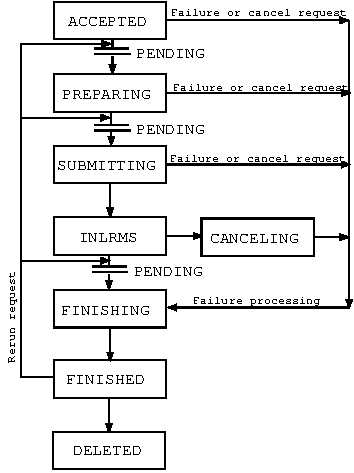
\includegraphics{pic1.pdf}
\caption{\label{job states diagram}Job states}
\end{figure}

A user can examine the state of a job by querying the dedicated Local
Information Description Interface of A-REX using the UI or any other
suitable tool or through query method of WS interface. 

Configuration can put limits on the amount of simultaneous jobs in
some states. If such a limit is reached, a job ready to enter into
the state in question will stay in it's current state waiting for
a free slot. This situation is presented by additional state mark
\textbf{PENDING} to the current state name in the job's status description.

Below is the description of all actions taken by the A-REX at every
state:

\begin{itemize}
\item \textbf{Accepted} -- In this state the job has been submitted to a
CE but is not processed yet. The A-REX will analyze the JD and move
to the next stage. If the JD can not be processed the job will be
canceled and moved to the state \textbf{Finishing}.
\item \textbf{Preparing} -- The input data is being gathered in the SD (stage-in).
The A-REX is downloading the files specified in the JD and is waiting
for files which are supposed to be uploaded by the UI. If all files
are successfully gathered the job moves to the next state. If \textbf{any}
file can't be downloaded or it takes the UI too long to upload a file,
the job moves to \textbf{Finishing} state. It is possible to put a
limit on the number of simultaneous \textbf{Preparing} jobs. 
If this limit is exceeded, jobs ready to enter the \textbf{Preparing} state
 will stay in the \textbf{Accepted} state, but prefixed with the PENDING:
mark. Exceptions are jobs which have no files to be downloaded. These
are processed out of limits.
\item \textbf{Submitting} -- The job is being passed for execution to the
\emph{Local Resource Management System} (LRMS). The corresponding
backends for many LRMSs are provided with the default installation.
If the local job submission is successful the job moves to the \textbf{Executing}
state. Otherwise it moves to \textbf{Finishing}. It is possible to
limit the aggregate number of jobs in \textbf{Submitting} and \textbf{Executing}
states.
\item \textbf{Executing} -- The job is queued or being executed in the LRMS.
The A-REX takes no actions except waiting until the job finishes.
\item \textbf{Killing} -- Necessary action to cancel the job in the LRMS
is being taken.
\item \textbf{Finishing} -- The output data is being processed (stage-out).
Specified data files are moved to the specified SEs and are optionally
registered at an Indexing Service. The user can download data files
from the SD by using the UI or other adequate tool. All the files
not specified as output files are removed from the SD at very beginning
of this state.It is possible to limit the number of simultaneous jobs in this state.
\item \textbf{Finished} -- No more processing is performed by the A-REX.
The user can continue to download data files from the SD. The SD is
kept available for some time (default is 1 week). After that the job
is moved to the state \textbf{Deleted}. The 'deletion' time can be
obtained by querying the Information Interface of the A-REX. If a
job was moved to \textbf{Finished} because of failure, it may be restarted
on request of a client. When restarted, a job is moved to the state
previous to the one in which it failed and is assigned mark PENDING.
This is needed in order to not break the configuration limits. Exception
is a job failed in \textbf{Executing} state and lacking input files
specified in JD. Such a job is treated like failed in \textbf{Preparing}
state.
\item \textbf{Deleted} -- The job is moved to this state if the user have
not requested job to be cleaned before the SD's lifetime expires.
Only minimal subset of information about such job is kept. The SD
is not available anymore.
\end{itemize}
In case of a failure special processing is applied to output files.
All specified output files are treated as \textbf{downloadable by
the user}. No files will be moved to their destination SE.

\section{URLs\label{sec:urls}}

In full installation the A-REX and it's components support the following
data transfer protocols and corresponding URLs: \emph{ftp, gsiftp,
http, https, lfc, rls} and \emph{srm.} For more information please see
{}``The Hosting Environment of the Advanced Resource Connector middleware''
document~\cite{hed}.

\section{Internals\label{section:internals}}

\subsection{Internal Files of the A-REX}

For each local UNIX user listed in the A-REX configuration -- including
a generic one which covers all local user identities -- a \textit{control
directory} exists. In this directory the A-REX stores information
about jobs belonging to that user. Multiple users can share the same
\textit{control directory}. In most common configuration case A-REX
serves all users defined by the Operating System and stores their control
files in the same directory. To make it easier to recover in case of failure,
the A-REX stores most information in files rather than in memory.
All files belonging to the same job have names starting with \textbf{job.ID.,}
where ID is the job identifier.

The files in the control directory and their formats are described
below:

\begin{itemize}
\item \textit{job.ID.status} -- current state of the job. This is a plain
text file containing a single word representing the internal name
of current state of the job. Possible values and corresponding external
job states are:

\begin{itemize}
\item ACCEPTED
\item PREPARING
\item SUBMIT
\item INLRMS
\item FINISHING
\item FINISHED
\item CANCELING
\item DELETED
\end{itemize}
\end{itemize}

See Section~\ref{Section:Job Flow} for a description of the various
states. Additionally each value can be prepended the prefix {}``PENDING:''
(like PENDING:ACCEPTED, see Section~\ref{Section:Job Flow}). This
is used to show that a job is \emph{ready} to be moved to the next
state but it has to stay in it's current state \emph{only} because
otherwise some limits set in the configuration would be exceeded.

\begin{itemize}
\item \textit{job.ID.description} -- contains the description of the job
(JD).
\item \textit{job.ID.local} -- information about the job used by the A-REX.
It consists of lines of format \textit{{}``name = value''}. Not
all of them are always available. The following names are defined:

\begin{itemize}
\item \textit{subject} -- user certificate's subject, also known as the distinguished
name (DN)
\item \textit{starttime} -- GMT time when the job was accepted represented
in the Generalized Time format of LDAP 
\item \textit{lifetime} -- time period to preserve the SD after the job has
finished in seconds
\item \textit{cleanuptime} -- GMT time when the job should be removed from
the cluster and it's SD deleted in Generalized Time format
\item \textit{notify} -- email addresses and flags to send mail to about
the job specified status changes
\item \textit{processtime} -- GMT time when to start processing the job in
Generalized Time format
\item \textit{exectime} -- GMT time when to start job execution in Generalized
Time format
\item \textit{expiretime} -- GMT time when the credentials delegated to the
job expire in Generalized Time format
\item \textit{rerun} -- number of retries left to rerun the job
\item \textit{jobname} -- name of the job as supplied by the user
\item \textit{projectname} -- name of the project as supplied by the user
\item \textit{lrms} -- name of the LRMS backend to be used for local submission
\item \textit{queue} -- name of the queue to run the job at
\item \textit{localid} -- job id in LRMS (appears only after the job has
reached state \textbf{InLRMS})
\item \textit{globalid} -- BES ActivityIdentifier XML tree, the global
identifier of the job
\item \textit{args} -- executable name followed by a list of command-line
arguments
\item \textit{downloads} -- number of files to download into the SD before
execution
\item \textit{uploads} -- number of files to upload from the SD after execution
\item \textit{gmlog} -- directory name which holds files containing information
about the job when accessed through GridFTP interface
\item \textit{clientname} -- name (as provided by the user interface) and
IP address:port of the submitting client machine
\item \textit{clientsoftware} -- version of software used to submit the job
\item \textit{sessiondir} -- the job's SD
\item \textit{failedstate} -- state in which job failed (available only if
it is possible to restart the job)
\item \textit{jobreport} -- URL of a user requested \emph{logger service}.
The A-REX will also send job records to this service in addition to
the default logger service configured in the configuration.
\item \textit{activityid} -- Job-id of previous job in case the job has been 
resubmitted or migrated. This value can appear multiple times if a job has been 
resubmitted or migrate more than once.
\item \textit{forcemigration} -- This boolean is only used for migration of jobs.
It determines whether the job should persist if the termination of the previous 
job fails.
\item \textit{transfershare} -- name of share used in \textbf{Preparing}
and \textbf{Finishing} states.
\end{itemize}

This file is filled partially during job submission and fully when
the job moves from the \textbf{Accepted} to the \textbf{Preparing}
state.

\item \textit{job.ID.input} -- list of input files. Each line contains 2
values separated by a space. First value contains name of the file
relative to the SD. Second value is a URL or a file description.
Example:


\hspace*{1cm}\textit{input.dat gsiftp://grid.domain.org/dir/input\_12378.dat}

A URL represents a location from which a file can be downloaded.
Each URL can contain additional options.

A file description refers to a file uploaded from the UI and consists
of {[}size]{[}.checksum] where

\hspace*{1cm}\textit{size} - size of the file in bytes.

\hspace*{1cm}\textit{checksum} - checksum of the file identical to
the one produced by \textbf{\textit{cksum}} (1).

These values are used to verify the transfer of the uploaded
file. Both size and checksum can be left out. A special kind of file
description {*}.{*} is used to specify files which are \textbf{not}
required to exist.

This file is used by the '\textbf{\textit{downloader}}' utility. Files
with \emph{URL} will be downloaded to the SD and files with 'file
description' will simply be checked to exist. Each time a new \textbf{valid}
file appears in the SD it is removed from the list and \textit{job.ID.input}
is updated. Any external tool can thus track the process of collecting
input files by checking \textit{job.ID.input.}

\item \textit{job.ID.output} -- list of output files. Each line contains
1 or 2 values separated by a space. First value is the name of the
file relative to the SD. The second value, if present, is a URL. Supported
URLs are the same as those supported by job.ID.input.

This file is used by the '\textbf{\textit{uploader}}' utility. Files
with \textit{URL} will be uploaded to SE and remaining files will
be left in the SD. Each time a file is uploaded it is removed from
the list and \textit{job.ID.output} is updated. Files not mentioned
as output files are removed from the SD at the the beginning of the
\textbf{Finishing} state.

\item \textit{job.ID.failed} -- the existence of this file marks the failure
of the job. It can also contain one or more lines of text describing
the reason of failure. Failure includes the return code different
from zero of the job itself.
\item \textit{job.ID.errors} -- this file contains the output produced by
external utilities like \textbf{\textit{downloader}}, \textbf{\textit{uploader}},
script for job submission to LRMS, etc on their stderr handle. Those
are not necessarily errors, but can be just useful information about
actions taken during the job processing. In case of problem include
content of that file while asking for help.
\item \textit{job.ID.diag} -- information about resources used during execution
of job and other information suitable for diagnostics and statistics.
It's format is similar to that of \textit{job.ID.local}. The following
names are at least defined:
\begin{itemize}
\item \textit{nodename} -- name of computing node which was used to execute
job,
\item \textit{runtimeenvironments} -- used runtime environments separated
by ';',
\item \textit{exitcode} -- numerical exit code of job,
\item \textit{frontend\_distribution} -- name and version of operating system
distribution on frontend computer,
\item \textit{frontend\_system} -- name of operating on frontend computer,
\item \textit{frontend\_subject} -- subject (DN) of certificate representing
frontend computer,
\item \textit{frontend\_ca} -- subject (DN) of issuer of certificate representing
frontend computer,
\end{itemize}
and other information provided by GNU \emph{time} utility. Note that
some implementation of \emph{time} insert unrequested information
in their output. Hence some lines can have broken format.
\item \textit{job.ID.proxy} -delegated X509 credentials.
\item \textit{job.ID.proxy.tmp} -- temporary X509 credentials with different
UNIX ownership used by processes run with effective \emph{user id}
different form job owner's \emph{id}.
\end{itemize}

There are other files with names like job.ID.{*} which are created
and used by different parts of the A-REX. Their presence in the \textit{control
directory} can not be guaranteed and can change depending on changes
in the A-REX code.

\subsection{Web Service Interface}

A-REX Web Service Interface provides means to submit a description
of a computational job to a computing resource, to stage-in additional
data, to monitor and control processing of jobs, and obtain data produced
during the execution of a job. The WS Interface is built and deployed
inside the Hosting Environment Daemon (HED) infrastructure~\cite{hed}.

\subsubsection{Basic Execution Service Interface}

The job submission and control interface is based on a document produced
by the OGF OGSA Basic Execution Services (BES) Working Group~\cite{ogsa-bes}.

The exchange of SOAP messages is performed via HTTP(S). The BES interface
is represented by two port-types -- BES-Management and BES-Factory.
The former is made to control the A-REX service itself and thus defines
operations to start and stop the functionality of the BES service.
The A-REX does not implement remote control of service functionality.
Hence the BES-Management port-type is not functional. The BES-Factory
port-type provides operations to submit new jobs (to create an activity
in terms of BES) and to monitor its state. It also has an ability
to provide information about the service. A-REX fully implements the
functionality of this port-type.

For job descriptions A-REX accepts the Job Submission Description
Language (JSDL)~\cite{jsdl} documents as defined by the OGF Job Submission
Description Language Working Group. Supported elements and extensions
are described below.

\subsubsection{Extensions to OGSA BES interface}

A-REX introduces two new operations in addition to those provided by
BES. It does that by defining its own port-type with new operations
\emph{ChangeActivityStatus} and \emph{MigrateActivity}(see 
Appendix~\ref{annex:arex-wsdl}).

The \emph{ChangeActivityStatus} operation provides a way to request 
simple transfers between states of jobs and corresponding
actions.

\begin{itemize}
\item \emph{ChangeActivityStatus}
\begin{itemize}
\item Input
\begin{itemize}
\item \emph{ActivityStatusType OldStatus}: Description of the state the
job is supposed to be in during execution of this request. If the
current state of the job is different from the one having been given,
the operation is aborted and a fault is returned. This parameter is
optional.
\item \emph{ActivityStatusType NewStatus}: Description of the state the
job is to be put into.
\end{itemize}
\item Output
\begin{itemize}
\item \emph{ActivityStatusType NewStatus}: Description of the current state
of the job.
\end{itemize}
\item Fault(s)
\begin{itemize}
\item \emph{NotAuthorizedFault}: Indicates that the client is not allowed
to do this operation.
\item \emph{InvalidActivityIdentifierFault}: There is no such job/activity.
\item \emph{CantApplyOperationToCurrentStateFault}: The requested transition
is not possible.
\end{itemize}
\end{itemize}

On result of this command, the job should be put into the requested
state. If such a procedure cannot be performed immediately then the
corresponding sequence is initiated and fault 
OperationWillBeAppliedEventuallyFault will be returned.

Since BES allows implementations to extend their initial activity
states with additional sub-states, A-REX defines a set of sub-states
of activity processing in addition to those defined by the BES, as
listed in Table~\ref{tab:Job-states-definitions}. Their meaning is
described in Section~\ref{Section:Job Flow}.

The \emph{MigrateActivity} operation generates a request to migrate a 
grid job from another ARC1 cluster, i.e. the operation will get input 
files and possibly job description from the cluster currently holding 
the job and create the job as a new activity at the present cluster.
Currently only migration of queuing jobs is supported. 

\item \emph{MigrateActivity}
\begin{itemize}
\item Input
\begin{itemize}
\item \emph{wsa:EndpointReferenceType ActivityIdentifier}: This 
element should contain the \emph{wsa:EndpointReference} of the job to 
be migrated.
\item \emph{ActivityDocument}: JSDL document of the job to be 
migrated. This element is optional.
\item \emph{Boolean ForceMigration}: Boolean that determines whether 
the job will persist on the new cluster if the termination of the 
previous job fails.
\end{itemize}
\item Output
\begin{itemize}
\item \emph{wsa:EndpointReferenceType ActivityIdentifier}: This 
element should contain the \emph{wsa:EndpointReference} of the new 
activity.
\item \emph{ActivityDocument}: Contains the JSDL document of the new 
activity.
\end{itemize}
\item Fault(s)
\begin{itemize}
\item \emph{NotAuthorizedFault}: Indicates that the client is not allowed
to do this operation.
\item \emph{NotAcceptingNewActivitiesFault}: A fault that indicates that A-REX 
currently is not accepting new activities.
\item \emph{UnsupportedFeatureFault}: This fault indicates that an sub-element in the 
JDSL document is not supported or the ActivityDocument has not been recognised as JSDL. 
\item \emph{InvalidRequestMessageFault}: This fault indicates that an element in the 
request is either missing or has an invalid format. Typically this would mean that 
the job-id cannot be located in the ActivityIdentifier of the old job.
\end{itemize}
\end{itemize}
\end{itemize}

The \emph{ActiviterIdentifier} specifies the URL of the job which will be migrated. In case the 
\emph{ActivityDocument} is filled this document will be used to create a new activity otherwise 
an attempt will be made to retrieve the job description through the BES operation
\emph{GetActivityDocument}.

Once the input files have been downloaded from the other cluster, a request will be send 
to terminate the old job. If this request fails the new activity at the present cluster 
will be terminate unless the \emph{ForceMigration} is true. This is to prevent the job 
from being executed at two different places at the same time.

%
\begin{table}

\caption{\label{tab:Job-states-definitions}Job states definitions and mappings}

\begin{tabular}{|>{\centering}p{0.15\columnwidth}|>{\centering}p{0.15\columnwidth}|>{\centering}p{0.2\columnwidth}|p{0.4\columnwidth}|}
\hline 
Applicable BES State&
ARC Sub-state&
A-REX internal state&
Description\tabularnewline
\hline
\hline 
\multirow{2}{*}{Pending}& Accepting& ACCEPTED &
Job is in the process of being submitted. This state is not recognised
by the A-REX yet. \emph{Accepted} is first reported state\\ \cline{2-4}
&Accepted& ACCEPTED& Job was submitted\\ \hline 
\multirow{8}{*}{Running}& Preparing& PREPARING& Stage-in process is going on\\ \cline{2-4} 
&Prepared& PREPARING + PENDING& Stage-in process has finished\\ \cline{2-4} 
&Submitting& SUBMIT& Communication with local batch system is in process\\ \cline{2-4} 
&Queued& INLRMS&
Job entered local batch system but is not runnning now. This state
is not recognised by the A-REX yet. \emph{Executing} is reported instead\\ \cline{2-4} 
&Executing& INLRMS& Job is being executed in local batch system\\ \cline{2-4} 
&Executed& INLRMS, INLRMS + PENDING&
Job execution in local batch system has finished. The A-REX dos not
detect job states inside local batch system yet. As result this state
is reported only if job is \emph{Pending}.\\ \cline{2-4} 
&Killing& CANCELING& Communication with local batch system to terminate execution is in process\\ \cline{2-4} 
&Finishing& FINISHING& Stage-out process is going on\\ \hline 
Cancelled& Killed& FINISHED&
Job was stopped by explicit user request. The A-REX currently does
not remember this request. \emph{Failed} is reported instead.\\ \hline 
Failed& Failed& FINISHED& There was a failure during execution\\ \hline 
Finished& Finished& FINISHED& Job finished successfully\\ \hline 
Finished& Deleted& DELETED& Job finished and was left in A-REX too long\\ \hline 
All& Pending& PENDING&
Job is prevented from going to the next state due to some internal
limits; this sub-state appears in parallel with other sub-states\\ \hline 
All& Held& &
Job processing is suspended on client request; this sub-state appears
in parallel with other sub-states. This state is reserved for future
and is not implemented yet.\\ \hline
\end{tabular}
\end{table}

\subsubsection{Delegation Interface}

The A-REX also supports the Delegation Interface (see Appendix~\ref{annex:delegation-wsdl}).
This is a common purpose interface to be used by ARC services which
accepts delegated credentials from clients. The Delegation Interface
implements two operations: initialization of credentials delegation
(DelegateCredentialsInit) and update/renewal of credentials (UpdateCredentials).

\begin{itemize}
\item \emph{DelegateCredentialsInit} operation -- this operation performs
the first half of the credentials delegation sequence.
\begin{itemize}
\item Input
\begin{itemize}
\item None. On this request the service generates a pair of \emph{public}
and private keys. The public key is then sent to the client in response.
\end{itemize}
\item Output(s)
\begin{itemize}
\item \emph{TokenRequestType TokenRequest}: Contains the public key generated
by the service as a Value element. It also provides an identifier
in the Id element which should be used to refer to the corresponding
private key.
\end{itemize}
\item Fault(s)
\begin{itemize}
\item \emph{UnsupportedFault}: Indicates that the service does not support
this operation despite supporting the port-type.
\item \emph{ProcessingFault}: Internal problems during generation of the
token.
\end{itemize}
\end{itemize}
\item \emph{UpdateCredentials} operation -- this operation makes it possible
to update the content of delegated credentials (like in the case of
credentials being renewed) unrelated to other operations of the service.
\begin{itemize}
\item Input
\begin{itemize}
\item \emph{DelegatedTokenType DelegatedToken}: Contains an X509 proxy certificate
based on the public key from the DelegateCredentialsInit signed by
the user's proxy certificate. Also includes the Id element which identifies
the private key stored at the service side associated with these credentials.
The reference element refers to the object to which these credentials
should be applied in a way specific to the service. The same element
must also be used for delegating credentials as part of other operations
on service.
\end{itemize}
\item Output(s)
\begin{itemize}
\item None.
\end{itemize}
\item Fault(s)
\begin{itemize}
\item \emph{UnsupportedFault}: Indicates that service does not support this
operation despite supporting the port-type.
\item \emph{ProcessingFault}: Internal problems during generation of the
token.
\end{itemize}
\end{itemize}
\end{itemize}

Additionally, A-REX Web Service Interface allows delegation to be
performed as part of the \emph{CreateActivity} operation of the BES-Factory
port-type. For this it accepts the element \emph{DelegatedCredentials}
inside the \emph{CreateActivity} element. The \emph{Id} element of
\emph{DelegatedCredentials} must contain an identifier obtained in
response to the previous \emph{DelegateCredentialsInit} operation.
For more information about delegations and delegation interface refer
to~\cite{wsrf-rp}.

\subsubsection{Local Information Description Interface}

The A-REX implements the Local Information Description Interface (LIDI)
interface common for all ARC services. This interface is based on
OASIS Web Services Resource Properties specification~\cite{wsrf-rp}.
Information about resources and maintained activities/jobs are represented
in a \emph{WS-Resource Properties} informational XML document. The
document type is defined in the A-REX WSDL as a \emph{ResourceInformationDocumentType}.
It contains the following elements/resources:

\begin{list}{--}{\setlength{\labelwidth}{0.5cm}\setlength{\rightmargin}{\leftmargin}}
\item [{\emph{nordugrid}}] -- description of computing resource that uses
NorudGrid LDAP schema~\cite{is} converted to XML document.
\item [{\emph{Domains}}] -- description of a computation resource
that uses Glue2 schema.
\end{list}
All information can be accessed either through requests on particular
resources or through XPath queries using WS-Resource Properties operations.

\subsubsection{Supported JSDL elements}

A-REX supports the following elements from the JSDL version 1.0 specification~\cite{jsdl}
including POSIX Applications extension and JSDL HPC Profile Application
Extension~\cite{jsdl-hpc}:

\begin{list}{--}{\setlength{\labelwidth}{0.5cm}\setlength{\rightmargin}{\leftmargin}}
\item [{\emph{JobName}}] -- name of the job as assigned by the user.
\item [{\emph{Executable}\ (POSIX,HPC)}] -- name of the executable file.
\item [{\emph{Argument}\ (POSIX,HPC)}] -- arguments the executable will
be launched with.
\item [{\emph{DataStaging}}]~
\begin{list}{--}{\setlength{\labelwidth}{0.5cm}\setlength{\rightmargin}{\leftmargin}}
\item [{Filename}] -- name of the data file on the executing node.
\item [{\emph{Source}}] -- source where the file will be taken from before
execution.
\item [{\emph{Target}}] -- destination the file will be delivered
to after execution.
\end{list}
\item [{\emph{Input}\ (POSIX,HPC)}] -- file to be used as standard input
for the executable.
\item [{\emph{Output}\ (POSIX,HPC)}] -- file to be used as standard output
for the executable.
\item [{\emph{Error}\ (POSIX,HPC)}] -- file to be used as standard error
for the executable.
\item [{\emph{MemoryLimit}\ (POSIX)}] -- amount of physical memory needed
for execution.
\item [{\emph{TotalPhysicalMemory}}] -- same as MemoryLimit.
\item [{\emph{IndividualPhysicalMemory}}] -- same as MemoryLimit.
\item [{\emph{CPUTimeLimit}\ (POSIX)}] -- maximal amount of CPU time needed
for execution.
\item [{\emph{TotalCPUTime}}] -- same as CPUTimeLimit.
\item [{\emph{IndividualCPUTime}}] -- same as CPUTimeLimit.
\item [{\emph{WallTimeLimit}\ (POSIX)}] -- amount of clock time needed
for execution.
\item [{\emph{TotalCPUCount}}] -- number of CPUs needed for execution.
\item [{\emph{IndividualCPUCount}}] -- same as \emph{TotalCPUCount}.
\end{list}
%Environment(POSIX) -- environment variable.

\subsubsection{ARC-specific JSDL Extensions}

A-REX accepts JSDL documents having the following additional elements
(see Appendix~\ref{annex:jsdl-extension}):

\begin{list}{--}{\setlength{\labelwidth}{0.5cm}\setlength{\rightmargin}{\leftmargin}}
\item [{\emph{IsExecutable}}] -- marks file to become executable
after being delivered to the computing resource.
\item [{\emph{RunTimeEnvironment}}] -- specifies the name of the Runtime
Environment needed for job execution.
\item [{\emph{Middleware}}] -- request for specific middleware on the computing
resource frontend.
\item [{\emph{RemoteLogging}}] -- destination for the usage record
report of the executed job.
\item [{\emph{LocalLogging}}] -- name for the virtual directory available
through job interface and containing various debug information about
job execution.
\item [{\emph{AccessControl}}] -- ACL expression which describes the identities
of those clients who are allowed to perform operations on this job.
\item [{\emph{Notify}}] -- Email destination for notification of job state
changes.
\item [{\emph{SessionLifeTime}}] -- duration for the directory containing
job-related files to exist after the job finished executing.
\item [{\emph{JoinOutputs}}] -- specifies if standard output and standard
error channels must be merged.
\item [{\emph{Reruns}}] -- defines how many times a job is allowed
to rerun in case of failure.
\item [{\emph{CredentialServer}}] -- URL of MyProxy service which
may be used for renewing the expired delegated job credentials.
\item [{\emph{CandidateTarget}}] -- specifies host name and queue
of a computing resource.
\item [{\emph{OldJobID}}] -- specifies the previous job-ids in case the job 
has been resubmitted or migrated.
\end{list}

\section{Cache\label{sec:cache}}

The A-REX can cache input files, so that subsequent jobs requiring the
same files do not have to download them again. Caching is enabled if
one or more cache directories are specified in the configuration
file. All input files except files uploaded by the user during job
submission are cached by default. This includes excutable files
downloaded by the A-REX. Caching can be explicitly turned off by the
user in the job description (see~\cite{userguide1}). The disk space
occupied by the cache is controlled by removing files in the order of
least recent access. For more information on configuration see
Section~\ref{SubSection:ConfigFile}.

\subsection{Structure}

Cached files are stored in sub-direcories under the \emph{data} directory
in each main cache directory. Filenames are constructed from an SHA-1
hash of the URL of the file, and split into subdirectories based on
the two initial characters of the hash. This enables the cached files
to be evenly split over a number of subdirectories. If
more than one cache directory is used the initial letter of the hash
also determines which cache is to be used. The algorithm is simply
to use the cache directory at index \emph{i} in the list of directories,
where \emph{i} is found from the initial letter of the hash mod the
number of caches. This limits the maximum number of cache directories
to 16, as SHA-1 hashes use the character set {[}\emph{0-9,a-f}]. In
the extremely unlikely event of a collision between two URLs having
the same SHA-1 hash, caching will not be used for the second file.

There is no indexing system for the cache, and any cache filename
can be easily determined from a URL by using the same hashing algorithm
as the A-REX, e.g. the standard command line tool \emph{sha1sum. }The
cache directory used by a file can be determined from the initial
letter of the hash and the order of cache directories in the configuration
file. Some associated metadata (the corresponding URL and an expiry
time, if available) are stored in a file with the same name as the
cache file, with a \emph{.meta} suffix.

For example, with a cache directory \emph{/cache}, the file 

\begin{center}
\emph{lfc://atlaslfc.nordugrid.org//grid/atlas/file1 }\\
is mapped to\\
\emph{/cache/data/78/f607405ab1df6b647fac7aa97dfb6089c19fb3}
\par\end{center}

and the file \emph{/cache/data/78/f607405ab1df6b647fac7aa97dfb6089c19fb3.meta
}contains the original URL and an expiry time if one is available.

At the start of a file download, the cache file is locked, so that
it cannot be deleted and so that another download process cannot write
the same file simultaneously. This is done by creating a file with the
same name as the cache filename but with a \emph{.lock} suffix. This
file contains the process ID of the process and the hostname of the
host holding the lock. If this file is present, another process cannot
do anything with the cache file and must wait until the cache file
is unlocked (i.e. the \emph{.lock} file no longer exists). The lock
has a timeout of one day, so that stale locks left behind by a download
process exiting abnormally will eventually be cleaned up. Also, if
the process corresponding to the process ID stored inside the lock
is no longer running on the host specified in the lock, it is safe
to assume that the lock file can be deleted.


\subsection{How it works}

If a job requests an input file which can be cached or is allowed to
be cached, it is stored in the selected cache directory, and depending
on the configuration, either the file is copied to the SD or a hard
link is created in a per-job directory and a soft link is created in
the SD to there. The per-job directories are in the \emph{joblinks}
subdirectory of the main cache directory. The former option is advised
if the cache is on a file system which will suffer poor performance
from a large number of jobs reading files on it, or the file system
containing the cache is not accessible from worker nodes. The latter
option is the default option. The per-job directory is only readable
by the local user running the job, and the cache directory is readable
only by the A-REX user. This means that the local user cannot access
any other users' cache files. It also means that cache files can be
removed without needing to know whether they are in use by a currently
running job. Note that when running A-REX under a non-privileged user
account, all cache files will be owned and accessible by the same
user, and therefore modifyable by running jobs. This is potentially
dangerous and so cacheing should be used with caution in this case.

If the file system containing the cache is full and it is impossible
to free any space, the download fails and is retried without using
cacheing.

Before giving access to a file already in the cache, the A-REX
contacts the initial file source to check if the user has read
permission on the file. In order to prevent repeated checks on source
files, this authentication information is cached for a limited
time. On passing the check for a cached file, the user's DN is stored
in the \emph{.meta} file, with an expiry time equivalent to the
lifetime remaining for the user's proxy certificate. This means that
the permission check is not performed for this user for this file
until this time is up (usually several hours). File creation and
validity times from the original source are also checked to make sure
the cached file is fresh enough. If the modification time of the
source is later than that of the cached file, the file will be
downloaded again. The file will also be downloaded again if the
modification date of the source is not available, as it is assumed the
cache file is out of date. These checks are not performed if the DN is
cached and is still valid.

The A-REX checks the cache periodically. If the used space on the file
system containing the cache exceeds the high water-mark given in the
configuration file it tries to remove the least-recently accessed
files to reduce size to the low water-mark.

\subsection{Cache Administration}

The cache is cleaned automatically periodically (every 2 minutes) by
the A-REX to keep the size of each cache within the configured limits.
Files are removed from the cache if the total size of the cache is
greater than the configured limit. Files which are not locked are
removed in order of access time, starting with the earliest, until the
size is lower than the configured lower limit. If the lower limit
cannot be reached (because too many files are locked, or other files
outside the cache are taking up space on the file system), the
cleaning will stop before the lower limit is reached.

Since the limits on cache size are given as a percentage of space used
on the filesystem on which the cache is located, it is recommended
that each cache has its own dedicated file system. If the cache shares
space with other data on a file system, changes in the amount of
non-cache data will result in changes in the available cache space.

With large caches mounted over NFS and an A-REX heavily loaded with
data transfer processes, cache cleaning can become slow, leading to
caches filling up beyond their configured limits. For performance
reasons it may be advantageous to disable cache cleaning by the A-REX,
and run the \emph{cache-clean} tool independently on the machine
hosting the file system.

The following tools (installed in \emph{\$ARC\_LOCATION/libexec/arc})
exist to help with administration of the cache:

\begin{itemize}
\item \emph{cache-clean} - This tool is used periodically by the A-REX to
  keep the size of each cache within the configured
  limits.\\
  \emph{cache-clean -h} gives a list of options. The most
  useful option for administrators is \emph{-s}, which does not delete
  anything, but gives summary information on the files in the cache,
  including information on the ages of the files in the cache.\\
  It is not recommended to run \emph{cache-clean} manually to clean up
  the cache, unless it is desired to temporarily clean up the cache with
  different size limits to those specified in the configuration, or to
  improve performance by running it on the file system's local node as
  mentioned above.
\item \emph{cache-list} - This tool is used to list all files present
  in each cache. It simply reads through all the \emph{.meta }files
  and prints to stdout a list of all URLs stored in each cache and
  their corresponding cache filename, one per line.
\end{itemize}


\section{Files and directories\label{sec:files and directories}}

\subsection{Modules}

The A-REX consists of several separate modules. These are:

\begin{itemize}
\item \textit{libarex.so} -- The main module providing main functionality
and web interface. It is implemented as HTTP and SOAP service inside
HED. It is responsible for processing jobs, moving them through states
and running other modules.
\item \textit{downloader} -- This is a module responsible for gathering input
files in the SD. It processes the \textit{job.ID.input} file and updates
it.
\item \textit{uploader} -- This module is responsible for delivering output
files to the specified SEs and registration at an Indexing Service
(like RLS) as needed. It processes and updates the \textit{job.ID.output}
file.
\end{itemize}

%cache-register -- Utility to register cached data into an Indexing Service. It reads and modifies cache informational files old and new (as described in Section ). Configuration is read directly from the A-REX's configuration file (see Section ). It is run by the A-REX every 5 minutes.

%frontend-info-collector -- Utility to gather information about the frontend. It puts collected information into the job.ID.diag file.

\begin{itemize}
\item \emph{gm-kick} -- Sends a signal to the A-REX though a FIFO file to
wake it up. It's used to increase responsiveness of A-REX.
\item \emph{CEinfo.pl} -- Collects and generates information about computing
resource as XML document in NorduGrid and Glue 2 format.
\end{itemize}

The following modules are always run under the Unix account to which
a Grid user is mapped.

\begin{itemize}
\item \textit{smtp-send.sh} and \textit{smtp-send} -- These are the modules
responsible for sending e-mail notifications to the user. The format
of the mail messages can be easily changed by editing the simple shell
script \textit{smtp-send.sh}. 
\item \textit{submit-{*}-job} -- Here {*} stands for the name of the LRMS.
Currently supported LRMS are PBS/Torque, Condor, LoadLeveler, LSF, SLURM,
and SGE. Also \emph{fork} pseudo-LRMS is supported for testing purposes.
This module is responsible for job submission to the LRMS.
\item \textit{cancel-{*}-job} -- This script is for canceling jobs which
have been already submitted to the LRMS.
\item \textit{scan-{*}-job} -This shell script is responsible for notifying
the A-REX about completion of jobs. It's implementation for PBS uses
server logs to extract information about jobs. If logs are not available
it uses the less reliable \emph{qstat} command for that. Other backends
use different techniques.
\end{itemize}

In addition, there is also an administration utility:

\begin{itemize}
\item \textit{gm-jobs} -- prints a list of jobs available on the cluster
and the number of jobs in each state.\\
\hspace*{0.5cm}gm-jobs {[}-h] {[}-s] {[}-l] {[}-u uid] {[}-U name] {[}-c conf\_file] {[}-d control\_dir]\\
\hspace*{0.5cm}-h -- print short help,\\
\hspace*{0.5cm}-s -- print summary of jobs in each transfer share,\\
\hspace*{0.5cm}-l -- print more information about each job,\\
\hspace*{0.5cm}-u -- pretend utility is run by user with id \emph{uid},\\
\hspace*{0.5cm}-U -- pretend utility is run by user with name \emph{name},\\
\hspace*{0.5cm}-c -- use specified configuration file,\\
\hspace*{0.5cm}-d -- read information from specified control dir.
\end{itemize}


\subsection{Directories}

The A-REX is installed into a single installation point referred as
\$ARC\_LOCATION and the following sub-directories are used:

\begin{itemize}
\item[] \$ARC\_LOCATION/bin -- tools
\item[] \$ARC\_LOCATION/libexec -- program modules used by A-REX
\item[] /etc -- central configuration file -- location used by default
\item[] \$ARC\_LOCATION/lib/arc -- service module
\end{itemize}

The A-REX also uses following directories:

\begin{itemize}
\item \textit{session root directory} -- This is the directory in which a
user's SDs are created. It's location is configurable per UNIX user.
Several (or even all) users may share the same session root directory.\\
The A-REX needs to have permission to create new files and directories
in the session root directory. If A-REX is run under a dedicated user
account, that account needs full permissions in the \textit{session
root directory}.\\
If A-REX is run under the \emph{root} account, make sure \textit{session
root directory} resides on a file system which does not limit the
capabilities of the \emph{root} user (as does for example NFS with
\emph{root\_squash} option).\\
If there is a need to run A-REX under the \emph{root} account (to
be able to run jobs in LRMS under different users' accounts, for example)
but there is no way to provide a suitable \textit{session root directory,}
use the \emph{norootpower} command in configuration file. In that
case A-REX will use the identity of the local user to which a Grid
identity is mapped to access the \textit{session root directory}.
Hence those users will need full access there.\\
The A-REX creates SDs with proper ownership and permissions for the
local identity used to run a job. Some file systems require users
to have \emph{execute} permission on the \textit{session root directory}
in order to access any file or subdirectory there.\\
In order for jobs to access their input files, session root directories
should be shared across cluster nodes. Otherwise, LRMS-specific methods
must be used to transfer files to execution nodes. 
\end{itemize}

\begin{comment} (LRMS\_COMMENT) For more information see Section~\ref{sub:LRMS}.\end{comment}

\begin{itemize}
\item \textit{control directory} -- In this directory A-REX stores an information
about accepted jobs. It must have full permissions there.\\
A subdirectory called \textit{logs} is created there. It is used to
accumulate information about started and finished jobs. This information
is periodically sent to the desired \emph{logger service}(s). For
each job start and stop event, and for each logger service where that
event must be sent, a separate file is written. Once an event is sent,
the corresponding file is deleted.
\end{itemize}

\section{Configuration}

\subsection{Configuration of the A-REX\label{SubSection:ConfigFile}}

Due to historical reasons configuration of the A-REX is split into 2
parts. The small part is located inside HED configuration (see
Appendix~\ref{annex:arex-conf} for schema and description of supported
elements). This configuration refers to the file containing the main
part of the configuration. The default location of the main
configuration file is \textit{/etc/arc.conf}.

The configuration file can contain empty lines and comments in lines
starting with \#. It is separated into sections. Each section starts
with a string containing

\begin{shaded}
\verb|[section name/subsection name/subsubsection name]|
\end{shaded}

Each section continues until the next section or until the end of the
file. The configuration file can have commands for multiple
services/modules/programs. Each service has its own section named
after it. The A-REX uses the \emph{{[}grid-manager]} section. Some
services can make use of multiple subsections to reflect their
internal modular structure. Commands in section \emph{{[}common]}
apply to all services. Command lines have the format

\begin{shaded}
\verb|name=``arguments string''|
\end{shaded}
The following commands are defined:

Commands affecting the A-REX process and logging:

\begin{itemize}
\item \textbf{\textit{pidfile}}\textit{=path} -- specifies file where
  process id of A-REX process will be stored. Defaults to
  \emph{/var/log/arched.pid} if running as root and
  \emph{\$HOME/arched.pid} otherwise.
\item \textbf{\textit{logfile}}\textit{=path} -- specifies name of file
  for logging debug/informational output. Defaults to
  \emph{/var/log/grid-manager.log}.
\item \textbf{\textit{logsize}}\textit{=size number} -- restricts
  log file size to \emph{size} and keeps \emph{number} archived log
  files.
\item \textbf{\textit{debug}}\textit{=number} -- specifies level of
  debug information. More information is printed for higher
  levels. Currently the highest effective number is 5 (DEBUG) and
  lowest 0 (FATAL). Defaults to 2 (WARNING).
\item \textbf{\textit{user}}\textit{=username} -- specifies username to
  which the A-REX must switch after reading configuration. Defaults to
  \emph{not switch}.
\end{itemize}

Commands setting limits and options for how the A-REX handles jobs and
files:

\begin{itemize}
\item \textbf{\textit{joblog}}\textit{=path} -- specifies where to store
log file containing information about started and finished jobs.
\item \textbf{\textit{jobreport}}\textit{=URL ... number} -- specifies
that A-REX has to report information about jobs being processed (started,
finished) to a centralized service running at the given \textit{URL}. Multiple
entries and multiple URLs are allowed. \textit{number} specifies how
long (in days) old records have to be kept if failed to be
reported. The last specified value becomes effective.
\item \textbf{\textit{jobreport\_credentials}}\textit{=key\_file
    {[}cert\_file {[}ca\_dir]]} -- specifies the credentials for
  accessing the accounting service.
\item \textbf{\textit{jobreport\_options}}\textit{=options}
  -- specifies additional options for Usage Reporter and/or
  accounting service. The \textit{options} string is interpreted by Usage
  Reporter, its format is described in the corresponding technical document.
\item \textbf{\textit{securetransfer}}\textit{=yes|no} -- specifies whether
to use encryption while transferring data. Currently works for GridFTP
only. Default is \emph{no}. It is overridden by values specified in
URL options.
\item \textbf{\textit{passivetransfer}}\textit{=yes|no} -- specifies
  whether GridFTP transfers are passive. Setting this option to yes
  can solve transfer problems caused by firewalls. Default is no.
\item \textbf{\textit{localtransfer}}\textit{=yes|no} -- specifies whether
to pass file downloading/uploading task to computing node. If set
to yes the A-REX will not download/upload files but compose script
submitted to the LRMS in order that the LRMS can execute file tranfer. This
requires installation of A-REX and all related software to be accessible
from computing nodes and environment variable ARC\_LOCATION to be
set accordingly. Default is \emph{no}.
\item \textbf{\textit{maxjobs}}\textit{={[}max\_processed\_jobs {[}max\_running\_jobs]]}
-- specifies maximum number of jobs being processed by the A-REX at
different stages:\\
\textit{max\_processed\_jobs} -- maximum number of concurrent jobs
processed by A-REX. This does not limit the amount of jobs, which can
be submitted to the cluster.\\
\textit{max\_running jobs} -- maximum number of jobs passed to Local
Resource Management System\\
Missing value or -1 means no limit.
\item \textbf{\textit{maxload}}\textit{={[}max\_frontend\_jobs {[}emergency\_frontend\_jobs
{[}max\_transferred\_files]]]} -- specifies maximum load caused by
jobs being processed on frontend:\\
\textit{max\_frontend\_jobs} -- maximum number of jobs in PREPARING and
FINISHING states (downloading and uploading files). Jobs in these
states can cause a heavy load on the A-REX host. This limit is applied
before moving jobs to PREPARING and FINISHING states.\\
\textit{emergency\_frontend\_jobs} -- if limit of \textit{max\_frontend\_jobs}
is used only by PREPARING or by FINISHING jobs, aforementioned number
of jobs can be moved to another state. This is used to avoid the case
where jobs cannot finish due to a large number of recently submitted jobs.\\
\textit{max\_transferred\_files} -- maximum number of files being transferred
in parallel by every job. Used to decrease load on not so powerful
frontends.\\
Missing value or -1 means no limit.
\item \textbf{\textit{maxloadshare}}\textit{=max\_share share\_type} -- specifies a 
sharing mechanism for data transfer. \emph{max\_share} is the maximum
number of processes that can run per transfer share and \emph{share\_type} is 
the scheme used to assign jobs to transfer shares. See Section~\ref{sub:Transfershare}
for possible values and more details.
\item \textbf{\textit{wakeupperiod}}\textit{=time} -- specifies how often
the A-REX checks for job state changes (like new arrived job, job
finished in LRMS, etc.). \textit{time} is a minimal time period specified
in seconds. Default is \emph{3 minutes}. The A-REX may also be woken up by
external processes such as LRMS scripts before this time period expires.
\item \textbf{\textit{authplugin}}\textit{=state options plugin} -- specifies
\emph{plugin} (external executable) to be run every time job is about
to switch to \emph{state}. The following states are allowed: ACCEPTED,
PREPARING, SUBMIT, FINISHING, FINISHED and DELETED. If exit code is
not 0 job is canceled by default. \textit{Options} consists of \textit{name}=\textit{value}
pairs separated by commas. The following \textit{name}s are supported:\\
\textit{timeout} -- specifies how long in seconds execution of the
plugin allowed to last (mandatory, {}``\textit{timeout=}{}`` can
be skipped for backward compatibility).\\
\textit{onsuccess}, \textit{onfailure} and \textit{ontimeout} -- defines
action taken in each case (\textit{onsuccess} happens if exit code
is 0). Possible actions are:\\
\textit{pass} -- continue execution,\\
\textit{log} -- write information about result into log file and continue
execution,\\
\textit{fail} -- write information about result into log file and cancel
job.
\item \textbf{\textit{localcred}}\textit{=timeout plugin} -- specifies \emph{plugin}
(external executable or function in shared library) to be run every
time job has to do something on behalf of local user. Execution of
\emph{plugin} may not last longer than \emph{timeout} seconds. If
\emph{plugin} looks like \emph{function@path} then function \emph{int
function(char{*},char{*},char{*},...)} from shared library \emph{path}
is called (\emph{timeout} is not functional in that case). If exit
code is not 0 current operation will fail.
\item \textbf{\textit{norootpower}}\textit{=yes/no} -- if set to \emph{yes}
all processes involved in job management will use local identity of
a user to which Grid identity is mapped in order to access file system
at path specified in \textbf{\textit{session}} command (see below).
Sometimes this may involve running temporary external process.
\item \textbf{\textit{speedcontrol}}\textit{=min\_speed min\_time min\_average\_speed
max\_inactivity} -- specifies how long/slow data transfer is allowed
to take place. Transfer is canceled if transfer rate (bytes per second)
is lower than \emph{min\_speed} for at least \emph{min\_time} seconds,
or if average rate is lower than \emph{min\_average\_speed}, or no
data is received for longer than \textit{max\_inactivity} seconds. To
allow statistics to build up, no transfers will be stopped within the
first 3 minutes.
\item \textbf{\textit{copyurl}}\textit{=template replacement} -- specifies
that URLs starting from \emph{template} should be accessed in a different
way (most probably Unix open). The \textit{template} part of the URL
will be replaced with \textit{replacement.} \textit{replacement} can
be either URL or local path starting from '/'. It is advisable to
end template with '/'.
\item \textbf{\textit{linkurl}}\textit{=template replacement {[}node\_path]}
-- mostly identical to \textit{copyurl} but file will not be copied. Instead
a soft-link will be created. \textit{replacement} specifies the way
to access the file from the frontend, and is used to check permissions.
The \textit{node\_path} specifies how the file can be accessed from
computing nodes, and will be used for soft-link creation. If \textit{node\_path}
is missing, \textit{local\_path} will be used instead. Neither \textit{node\_path}
nor \textit{replacement} should be URLs.
\begin{framed}
NOTE: URLs which fit into \textit{copyurl} or \textit{linkurl} are
treated as more easily accessible than other URLs. That means if A-REX
has to choose between several URLs from which should it download input
file, these will be tried first.
\end{framed}
\end{itemize}

Per UNIX user commands

\begin{itemize}
\item \textbf{\textit{mail}}\textit{=e-mail\_address} -- specifies an email
address \textbf{from} which notification mails are sent.
\item \textbf{\textit{defaultttl}}\textit{=ttl {[}ttr]} -- specifies the
time in seconds for the SD to be available after job finishes (\emph{ttl})
and after job was deleted (\emph{ttr}) due to \emph{ttl}. Defaults
are 7 days for \emph{ttl} and 30 days for \emph{ttr}. The minumum value
for both parameters is 2 hours.
\item \textbf{\textit{lrms}}\textit{=default\_lrms\_name default\_queue\_name}
-- specifies names for the LRMS and queue. Queue name can also be specified
in the JD (currently it is not allowed to override LRMS by using
the JD).
\item \textbf{\textit{sessiondir}}\textit{=path} -- specifies path to
  the directory in which the SD is created. If \emph{path} is {*} the
  default sessiondir is used -- \textit{\$HOME/.jobs}.
\item \textbf{\textit{cachedir}}\textit{=path {[}link\_path]} -- specifies
a directory to store cached data (see section \ref{sec:cache}). Multiple
cache directories may be specified by specifying multiple \emph{cachedir}
commands. Cached files will be distributed evenly between the caches.
Specifying no \emph{cachedir }command or commands with an empty path
disables caching. Optional \textit{link\_path} specifies the path
at which \emph{path} is accessible on computing nodes, if it is different
from the path on the A-REX host. If \textit{link\_path} is set to '.'
files are not soft-linked, nor are per-job links created, but files
are copied to the session directory.
\item \textbf{\textit{cachesize}}\textit{=high\_mark {[}low\_mark]} --
  specifies high and low watermarks for space used on the file system
  on which the cache directory is located, as a percentage of total
  file system capacity. When the max is exceeded, files will be
  deleted to bring the used space down to the min level. It is a good
  idea to have each cache on its own separate file system. To turn off
  this feature, \char`\"{}cachesize\char`\"{} without parameters can
  be specified. These cache settings apply to all caches specified by
  \emph{cachedir} commands.
\item \textbf{\textit{maxrerun}}\textit{=number} -- specifies maximal number
of times job will be allowed to rerun after it failed at any stage.
Default value is \emph{5}. This only specifies a upper limit. The actual
number is provided in job description and defaults to 0.
\end{itemize}

All per-user commands should be put before the \textit{control} command
which initiates serviced user.

\begin{itemize}
\item \textbf{\textit{control}}\textit{=path username {[}username
    {[}...]]} -- This option initiates UNIX user as being serviced by
  the A-REX.  \textit{path} refers to the control directory (see
  Section~\ref{section:internals} for the description of control
  directory). If the path is {*} the default one is used --
  \verb|$HOME/.jobstatus|. \textit{username} stands for UNIX name of
  the local user. Multiple names can be specified.  If the name is {*}
  it is substituted by all names found in file
  \texttt{/etc/grid-security/grid-mapfile} (for the format of this
  file one should study the Globus project~\cite{globus}).\\ Also the
  special name '.'(dot) can be used. Corresponding control directory
  will be used for \textbf{any} user. This option should be the last
  one in the configuration file. There is also command
  \textbf{\textit{controldir}}\textit{=path}.  It uses special
  username '.' and is always executed last independent of its
  placement in file.
\item \textbf{\textit{helper}}\textit{=username command {[}argument
    {[}argument {[}...]]]} -- associates an external program with the
  local UNIX user.  This program will be kept running under account of
  the user specified by \textit{username}. Special names can be used:
  '{*}' -- all names from /etc/grid-security/grid-mapfile, '.'  - root
  user. The user should be already configured with \textit{control}
  option (except root, who is always configured). \textit{command} is
  an executable and \textit{argument}s are passed as arguments to it.
\end{itemize}


The following are global commands specific to communication with the underlying
LRMS.

\begin{comment}

\begin{itemize}
\item \textbf{\textit{pbs\_bin\_path}}\textit{=path} -- path to directory
which contains PBS commands.
\item \textbf{\textit{pbs\_log\_path}}\textit{=path} -- path to directory
with PBS server's log files.
\end{itemize}
\end{comment}

\begin{itemize}
\item \textbf{\textit{gnu\_time}}\textit{=path} -- path to \emph{time}
  utility.
\item \textbf{\textit{tmpdir}}\textit{=path} -- path to directory for temporary
files.
\item \textbf{\textit{runtimedir}}\textit{=path} -- path to directory which
contains \emph{runtimenvironment} scripts.
\item \textbf{\textit{shared\_filesystem}}\textit{=yes|no} -- if computing
nodes have an access to session directory through a shared file system
like NFS. \begin{comment} Corresponds to an environment variable
RUNTIME\_NODE\_SEES\_FRONTEND (see Section~\ref{sub:LRMS}). \end{comment}
\item \textbf{\textit{nodename}}\textit{=command} -- command to obtain hostname
of computing node.
\item \textbf{\textit{scratchdir}}\textit{=path} -- path on computing node
where to move session directory before execution.
\item \textbf{\textit{shared\_scratch}}\textit{=path} -- path on frontend
where \textbf{\textit{scratchdir}} can be found.
\end{itemize}

In the command arguments (paths, executables, ...) following substitutions
can be used:

\begin{itemize}
\item [{\%R}] -- session root -- see command \emph{sessiondir}
\item [{\%C}] -- control dir -- see command \emph{control}
\item [{\%U}] -- username
\item [{\%u}] -- userid -- numerical
\item [{\%g}] -- groupid -- numerical
\item [{\%H}] -- home dir -- home specified in /etc/passwd
\item [{\%Q}] -- default queue -- see command \emph{lrms}
\item [{\%L}] -- default lrms -- ses command \emph{lrms}
\item [{\%W}] -- installation path -- \$\{ARC\_LOCATION\}
\item [{\%G}] -- globus path -- \$\{GLOBUS\_LOCATION\}
\item [{\%c}] -- list of all control directories
\item [{\%I}] -- job ID (for plugins only, substituted in runtime)
\item [{\%S}] -- job state (for \emph{authplugin} plugins only, substituted
in runtime)
\item [{\%O}] -- reason (for \emph{localcred} plugins only, substituted
in runtime). Possible reasons are:
\begin{list}{--}{\setlength{\labelwidth}{0.5cm}\setlength{\rightmargin}{\leftmargin}}
\item [{new}] -- new job, new credentials
\item [{renew}] -- old job, new credentials
\item [{write}] -- write/delete file, create/delete directory
\item [{read}] -- read file, directory, etc.
\item [{extern}] -- call external program 
\end{list}
\end{itemize}

\subsection{Transfer shares\label{sub:Transfershare}}

For many jobs, large amounts of input and output data can mean
significant time is spent in the PREPARING and FINISHING states
gathering input data and writing output data. With FIFO processing,
this can lead to one user or group of users blocking the queue for
others. The A-REX implements a sharing system to avoid this problem, by
assigning each user or group of users to a ``transfer share'' and
specifying a limit on the number of data transfer processes per
share. If one user's jobs' transfer share is using the maximum number
of processes and another user submits jobs which are assigned to a
different share, the second user's jobs can immediately go to
PREPARING, up to the same maximum limit of processes. This means that
no matter how many jobs the first user submits, the second user's jobs
are not blocked. Assuming the bandwidth from the sources of input data
for both users' jobs is similar, the available throughput will then be
split evenly between the two users' jobs.

If a limit on the total number of data transfer processes is set in
the \emph{maxload} option, the maximum number of processes per
transfer share is set by splitting the total maximum evenly among all
the shares with jobs in data transfer states, up to the maximum
allowed per share.

The scheme used to assign jobs to transfer shares can be set in the
\emph{maxloadshare} option. Possible values are:

\begin{itemize}
\item \emph{dn} - each job is assigned to a share based on the DN of
  the user sumbitting the job.
\item \emph{voms:vo} - if the user's proxy is a VOMS~\cite{voms} proxy
  the job is assigned to a share based on the VO specified in the
  proxy. If the proxy is not a VOMS proxy a default share is used.
\item \emph{voms:role} - if the user's proxy is a VOMS proxy the job
  is assigned to a share based on the role specified in the first
  attribute found in the proxy. If the proxy is not a VOMS proxy a
  default share is used.
\item \emph{voms:group} - if the user's proxy is a VOMS proxy the job is
  assigned to a share based on the group specified in the first
  attribute found in the proxy. If the proxy is not a VOMS proxy a
  default share is used.
\end{itemize}

If VOMS is not supported, the \emph{dn} scheme is the only option that
should be used, as using a VOMS-based scheme will lead to all jobs
being assigned to the default share. The current number of jobs
processing and pending processing for each share can be seen with the
command \emph{gm-jobs -s}.

\textbf{Important:} If a sharing mechanism based on VOMS is used,
server certificates for each supported VO must be installed. It is
possible to either download the public key of each VOMS server, or
create a special file for each VO containing the server's DN and its
CA DN. Instructions are given on NorduGrid's web site at
\url{http://www.nordugrid.org/documents/voms-notes.html}.

When XML file only is used to configure the A-REX, the transfer shares
can be implemented by defining \emph{maxLoadShare} (the limit itself)
and \emph{loadShareType} (the scheme used) elements inside 
\emph{loadLimits} block.

\subsection{Authorization\label{sub:Authorization}}

Authorization is performed by generic means provided by HED framework.
Currently A-REX does not implement any internal authorization techniques
except those imposed by Access Policy assigned to jobs through AccessControl
element of assigned JSDL.

\subsection{LRMS support\label{sub:LRMS}}

For information about supported LRMSes and their specific features
and configuration options please read dedicated documentation~\cite{arc1-backends}.

\begin{comment}(LRMS\_COMMENT) 

The A-REX comes with support for several LRMS. And this number is
slowly growing. Features explained below are for \textbf{PBS/Torque}
backend. This support is provided through \textit{submit-pbs-job},
\textit{cancel-pbs-job}, \textit{scan-pbs-job} scripts. \textit{submit-pbs-job}
creates job's script and submits it to PBS. Created job's script is
responsible for moving data between frontend machine and cluster node
(if required) and execution of actual job. Alternatively it can download
input files and upload output if \emph{{}``localtransfer=no''} is
specified in the configuration file.

Behavior of submission script is mostly controlled using environment
variables. Most of them can be specified on frontend in A-REX's environment
and overwritten on cluster's node through PBS configuration. Some
of them may be set in configuration file too.

\textbf{\textit{PBS\_BIN\_PATH}} -- path to PBS executables. Like \emph{/usr/local/bin}
for example. \emph{}Corresponds to \emph{pbs\_bin\_path} configuration
command.

\textbf{\textit{PBS\_LOG\_PATH}} -- path to PBS server logs. Corresponds
to \emph{pbs\_log\_path} configuration command.

\textbf{\textit{TMP\_DIR}} -- path to directory to store temporary
files. Default value is \emph{/tmp}. Corresponds to \emph{tmpdir}
configuration command.

\textbf{\textit{RUNTIME\_CONFIG\_DIR}} -- path where runtime setup
scripts can be found. Corresponds to \emph{runtimedir} configuration
command.

\textbf{\textit{GNU\_TIME}} -- path to GNU time utility. It is important
to provide path to utility compatible with GNU time. If such utility
is not available, modify \textit{submit-pbs-job} to either reset this
variable or change usage of available utility. Corresponds to \emph{gnu\_time}
configuration command.

\textbf{\textit{NODENAME}} -- command to obtain name of cluster's node.
Default is \emph{/bin/hostname -f}. Corresponds to \emph{nodename}
configuration command.

\textbf{\textit{RUNTIME\_LOCAL\_SCRATCH\_DIR}} -- if defined should
contain path to the directory on computing node, which can be used
to store job's files during execution. \emph{scratchdir} configuration
command.

\textbf{\textit{RUNTIME\_FRONTEND\_SEES\_NODE}} -- if defined should
contain path corresponding to \textit{}\\
\textit{RUNTIME\_LOCAL\_SCRATCH\_DIR} as seen on \textbf{frontend}
machine. Corresponds to \emph{shared\_scratch} configuration command.

\textbf{\textit{RUNTIME\_NODE\_SEES\_FRONTEND}} -- if set to {}``\emph{no}''
means computing node does not share file system with frontend. In
that case content of the SD is moved to computing node by using means
provided by the LRMS. Results are moved back after job's execution
in a same way. Corresponds to \emph{shared\_filesystem} configuration
command.

Figures~\ref{fig:no-node-scratch},~\ref{fig:node-scratch-not-vis-on-front},~\ref{fig:node-scratch-vis-on-front}
present some possible combinations for RUNTIME\_LOCAL\_SCRATCH\_DIR
and \\
RUNTIME\_FRONTEND\_SEES\_NODE and explain how data movement is performed.
Pictures a) correspond to the situation right after all input files
have been gathered in the session directory and show the actions taken
right after the job's script starts. Pictures b) show the situation
while the job is running and the actions which are taken right after
it has finished. Pictures c) illustrate the final situation, when
the job's output files are ready to be uploaded to an external storage
element or be downloaded by the user.

%
\begin{figure}[ht]
\begin{centering}
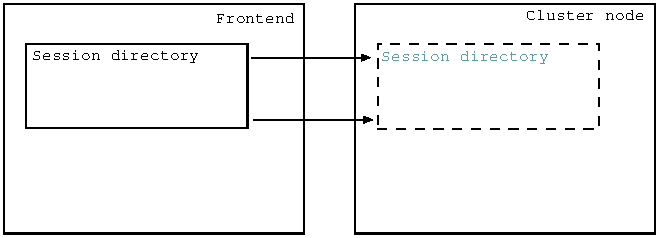
\includegraphics{pic2.pdf}
\end{centering}
\caption{\label{fig:no-node-scratch}Both RUNTIME\_LOCAL\_SCRATCH\_DIR and
RUNTIME\_FRONTEND\_SEES\_NODE are undefined. It is assumed that session
directories are visible from computing nodes. The job is executed
directly in the session directory prepared by the A-REX on the frontend.}
\end{figure}
%
\begin{figure}[ht]
\begin{centering}
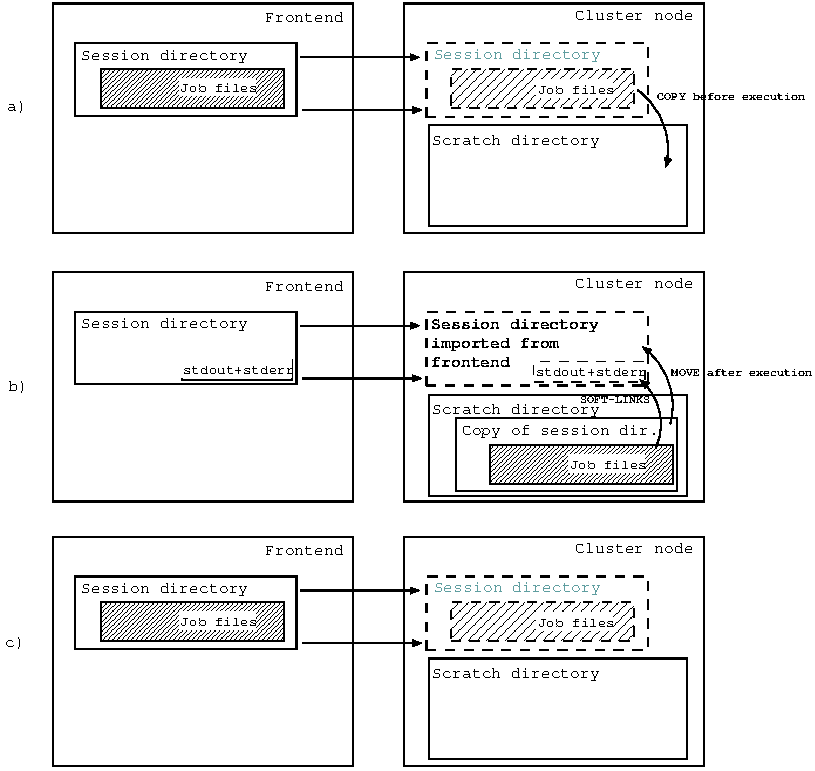
\includegraphics{pic3.pdf}
\end{centering}
\caption{\label{fig:node-scratch-not-vis-on-front}RUNTIME\_LOCAL\_SCRATCH\_DIR
is set to the location of the scratch directory on the computing node,
RUNTIME\_FRONTEND\_SEES\_NODE is undefined.}

\begin{itemize}
\item [{a)}] After the job script starts all the input files are moved to the 'scratch
directory' on the computing node.
\item [{b)}] The job runs in a separate directory in the 'scratch directory'.
Only the files representing the job's \textit{stdout} and \textit{stderr}
are placed in the original 'session directory' and soft-linked in
'scratch'. After execution all the files from 'scratch' are moved back
to the original 'session directory'.
\item [{c)}] All output files are in the 'session directory' and are ready
to be uploaded/downloaded.
\end{itemize}

\end{figure}
%
\begin{figure}[ht]
\begin{centering}
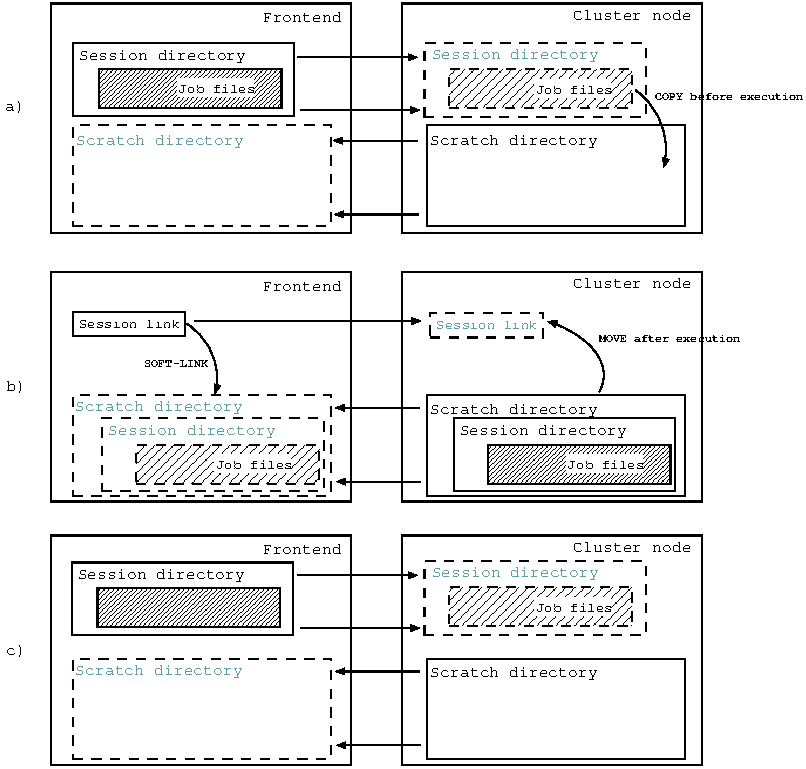
\includegraphics{pic4.pdf}
\end{centering}
\caption{\label{fig:node-scratch-vis-on-front}Both RUNTIME\_LOCAL\_SCRATCH\_DIR
and RUNTIME\_FRONTEND\_SEES\_NODE are set to the location of the scratch
directory on the computing node and the location where this scratch
directory is accessible from the frontend, respectively}.

\begin{itemize}
\item [{a)}] After the job script starts all input files are moved to the 'scratch
directory' on the computing node. The original 'session directory'
is removed and replaced with a soft-link to copy of session directory
in 'scratch directory' as seen on the frontend.
\item [{b)}] The job runs in a separate directory in 'scratch directory'.
All files are also available on frontend through the soft-link. After
execution the soft-link is replaced with a directory and all files
from 'scratch' are moved back to the original 'session directory'.
\item [{c)}] All output files are in the 'session directory' and are ready
to be uploaded/downloaded. 
\end{itemize}

\end{figure}

\end{comment}

\subsection{Runtime environment}

The A-REX can run specially prepared \emph{BASH} scripts prior to creation
of the job's script, before and after executing job's main executable.
Those scripts are requested by the user through the \emph{runtimeenvironment}
attribute in JSDL and are run with the only argument set either equal to '0',
'1' or '2' during creation of the job's script, before execution of the main
executable and after main the executable is finished, respectively. They all
are run through BASH's 'source' command, and hence can manipulate
shell variables. With argument '0' scripts are run by the A-REX on the
frontend. Some environment variables are defined in that case and
can be changed to influence job's execution later:

\begin{itemize}
\item joboption\_directory -- session directory.
\item joboption\_arg\_\# -- command with arguments to be executed as specified
in the JD (\textbf{not} bash array).
\item joboption\_env\_\# -- array of 'NAME=VALUE' environment variables (\textbf{not}
bash array).
\item joboption\_runtime\_\# -- array of requested \emph{runtimeenvironment}
names (\textbf{not} bash array).
\item joboption\_num -- \emph{runtimeenvironment} currently beeing processed
(number starting from 0).
\item joboption\_stdin -- name of file to be attached to stdin handle.
\item joboption\_stdout -- same for stdout.
\item joboption\_stderr -- same for stderr.
\item joboption\_cputime -- amount of CPU time requested (minutes).
\item joboption\_memory -- amount of memory requested (megabytes).
\item joboption\_count -- number of processors requested.
\item joboption\_lrms -- LRMS to be used to run job.
\item joboption\_queue -- name of a queue of LRMS to put job into.
\item joboption\_nodeproperty\_\# -- array of properties of computing nodes
(LRMS specific, \textbf{not} bash array).
\item joboption\_jobname -- name of the job as given by user.
\item joboption\_rsl -- whole RSL for very clever submission scripts.
\item joboption\_rsl\_\emph{name} -- RSL attributes and values (like joboption\_rsl\_executable=''/bin/echo'')
\end{itemize}

For example \emph{joboption\_arg\_\#} could be changed to wrap the main
executable. Or \emph{joboption\_runtime} could be expanded if current
one depends on others.

With argument '1' scripts are run just before the main executable is run.
They are executed on the computing node. Such a script can prepare environment
for some third-party software package. A current directory in that
case is the one which would be used for execution of the job. Variable \verb|$HOME|
also points to that directory.

With argument '2' scripts are executed after main executable finished.
Main purpose is to clean possible changes done by scripts run with
'1' (like removing temporary files). Execution of scripts at that
stage also happens on computing node and is not reliable. If the job
is killed by LRMS they most probably won't be executed.

For publicly available runtime environments please see the RTE repository at \url{http://gridrer.csc.fi/}.

\section{Installation\label{sec:installation}}

The A-REX is installed as an ARC1 component of ARC middleware and is available
in NorduGrid download area at ARC1 Download \url{http://download.nordugrid.org/software/nordugrid-arc1/}.There are packages available for various Linux distributions. The
A-REX comes in the \texttt{nordugrid-arc1-arex} package. Source code ready for
compilation is available too.

\subsection{Requirements}

When installed from binary packages, all the dependencies are handled automatically.
For compilation from source code please read included README files.


\subsection{Setup of the A-REX}

The A-REX service is a pluggable module of the HED, so it is first
required to set up HED configuration, and add the A-REX elements. To
add A-REX to an existing HED configuration, add a new \verb|<Name>|
element inside \verb|<Plugins>| containing the string
\emph{arex}. This will make HED load the libarex plugin library.

Then add a new \verb|<Service>| element with attribute
\verb|name="a-rex"|. That will instantiate the A-REX service. Now to
make service accessible extend the \verb|<Plexer>| element with new
\verb|<next>| referring to an id of the service. Take care to write
the \verb|<Service>| element carefully.

Here is an example of the full HED configuration file including the
A-REX service definition:

\begin{shaded}
\begin{verbatim}
<?xml version="1.0"?>
<ArcConfig
  xmlns="http://www.nordugrid.org/schemas/arcconfig/2009/08"
  xmlns:loader="http://www.nordugrid.org/schemas/loader/2009/08"
  xmlns:arex="http://www.nordugrid.org/schemas/a-rex/2009/08"
  xmlns:tcp="http://www.nordugrid.org/schemas/tcp/2009/08"
  xmlns:tls="http://www.nordugrid.org/schemas/tls/2009/08"
  xmlns:authz="http://www.nordugrid.org/schemas/arcauthz/2009/08"
  xmlns:idmap="http://www.nordugrid.org/schemas/identitymap/2009/10"
>
  <!-- Common configuration of the daemon -->
  <Server>
    <PidFile>/var/run/arched.pid</PidFile>
    <Logger>
      <Level>VERBOSE</Level>
      <File>/var/log/arched.log</File>
      <MaxSize>100000000</MaxSize>
      <Backups>10</Backups>
    </Logger>
  </Server>
  <!-- Where to find plugins -->
  <loader:ModuleManager>
    <loader:Path>/usr/local/lib/arc/</loader:Path>
  </loader:ModuleManager>
  <!-- Simply load all needed plugins -->
  <loader:Plugins>
    <loader:Name>mcctcp</loader:Name>
    <loader:Name>mcctls</loader:Name>
    <loader:Name>mcchttp</loader:Name>
    <loader:Name>mccsoap</loader:Name>
    <loader:Name>arcpdc</loader:Name>
    <loader:Name>identitymap</loader:Name>
    <loader:Name>arex</loader:Name>
  </loader:Plugins>
  <!-- Create a chain -->
  <loader:Chain>
    <!-- TCP listening socket -->
    <loader:Component name="tcp.service" id="tcp">
      <loader:next id="tls"/>
      <tcp:Listen><tcp:Port>60000</tcp:Port></tcp:Listen>
    </loader:Component>
    <!-- Transport-level security -->
    <loader:Component name="tls.service" id="tls">
      <loader:next id="http"/>
      <!-- Location of server's security keys -->
      <tls:KeyPath>/etc/grid-security/hostkey.pem</tls:KeyPath>
      <tls:CertificatePath>/etc/grid-security/hostcert.pem</tls:CertificatePath>
      <tls:CACertificatesDir>/etc/grid-security/certificates</tls:CACertificatesDir>
      <!-- Evaluate requestor's identity into local identity.
      Comment it if no user mapping is needed. -->
      <loader:SecHandler name="identity.map" id="map" event="incoming">
        <!-- Safe choice if all other rules failed -->
        <idmap:PDP name="allow.pdp"><idmap:LocalName>nobody</idmap:LocalName></idmap:PDP>
      </loader:SecHandler>
    </loader:Component>
    <!-- HTTP processing is done here -->
    <loader:Component name="http.service" id="http">
      <loader:next id="soap">POST</loader:next>
      <loader:next id="plexer">GET</loader:next>
      <loader:next id="plexer">PUT</loader:next>
    </loader:Component>
    <!-- This one parses content into XML tree -->
    <loader:Component name="soap.service" id="soap">
      <loader:next id="plexer"/>
    </loader:Component>
    <!-- Directing messages to proper service -->
    <loader:Plexer name="plexer.service" id="plexer">
      <!-- RegExp pattern is matched to path part of endpoint.
      Unmatched part of path is propagated to service in
      PLEXER:EXTENSION attribute. -->
      <loader:next id="a-rex">^/arex</loader:next>
    </loader:Plexer>
    <!-- A-Rex service -->
    <loader:Service name="a-rex" id="a-rex">
      <!-- Optional endpoint element is advised in case of multiple IP adresses -->
      <arex:endpoint>https://localhost:60000/arex</arex:endpoint>
      <!-- Use information generated by identity.map plugin or default provided below -->
      <arex:usermap><arex:defaultLocalName>nobody</arex:defaultLocalName></arex:usermap>
      <!-- grid-manager part of a-rex requires legacy configuration file.
      Use arc.conf example or write own. -->
      <arex:gmconfig>/etc/arc.conf</arex:gmconfig>
    </loader:Service>
  </loader:Chain>
</ArcConfig>
\end{verbatim}
\end{shaded}

For in-depth information about available elements see Appendix~\ref{annex:arex-conf}. 

For A-REX configuration, either use a template arc.conf or write a new
A-REX configuration file.  For information about format and available
configuration commands see Section~\ref{SubSection:ConfigFile}. It is
also possible to specify the A-REX configuration in XML format in the
HED configuration file, instead of a separate file. For more
information on this see the examples included in the documentation
bundled with the release.


\subsection{Usage}

For a quick start, simply run

\begin{shaded}
\begin{verbatim}
$ARC_LOCATION/sbin/arched -c <HED configuration file>
\end{verbatim}
\end{shaded}

For more information please read the \emph{User Guide}~\cite{userguide1}.

\subsection{Running as non-root}

The A-REX is primarily designed to be run by the \emph{root} UNIX
account and serve multiple global Grid identities mapped to several
UNIX accounts. Nevertheless it is possible to use \emph{non-root}
accounts to run that service at the cost of some functionality loss
as described below.

There are no drawbacks of running A-REX under a \emph{non-root} account
as long as the only UNIX identity used is that of the user who runs
the services and all served files and directories are owned by the
server's account. Because A-REX has to impersonate a user's local
account while communicating with the LRMS, it can serve only the account
it is run under (unless it is run under the \emph{root} account, of
course).

\appendix

\section{Session directory access through HTTP(S) interface\label{annex:a}}

In addition to the BES interface A-REX provides access to the SD through
pure HTTP(S) interface. This functionality is used for uploading user-stageable
files during job submission and for staging out result files produced
by job. It can also be used to monitor job execution by checking content
of application dependent files in SD.

The BES defines job identifier as WS Addressing~\cite{ws-addr-soap}
Endpoint Reference (EPR) -- XML document. The EPR is extendable and 
the A-REX adds it own element \texttt{JobSessionDir} belonging to the namespace
\texttt{http://www.nordugrid.org/schemas/a-rex} as a direct child of ReferenceParameters
element. This new element contains the URL of SD.

Obtained URL should be extended with file names relative to SD and
HTTP methods PUT and GET may be used to upload/download content of
those files. For directories -- including SD itself -- GET method is
supported which returns HTML encoded non-recursive list of files and
directories. The files and subdirectories have their URLs inside HTML
element \verb|<A>|.


\section{Configuration schema of A-REX\label{annex:arex-conf}}

\begin{footnotesize}
\begin{verbatim}
<?xml version="1.0" encoding="UTF-8"?>
<xsd:schema
xmlns:xsd="http://www.w3.org/2001/XMLSchema"
xmlns="http://www.nordugrid.org/schemas/ArcConfig/2007/arex"
xmlns:arc="http://www.nordugrid.org/schemas/ArcConfig/2007/arex"
targetNamespace="http://www.nordugrid.org/schemas/ArcConfig/2007/arex"
elementFormDefault="qualified">
  <xsd:complexType name="endpoint_Type">
    <!--
    This element defines URL of A-REX service as seen from outside.
    -->
    <xsd:simpleContent>
      <xsd:extension base="xsd:string"> 
      </xsd:extension>
    </xsd:simpleContent>
  </xsd:complexType>
  <xsd:element name="endpoint" type="endpoint_Type"/>
  <xsd:complexType name="gmconfig_Type">
    <!--
    This element defines path to arc0 Grid Manager configuartion file.
    By default it is /etc/arc.conf.
    -->
    <xsd:simpleContent>
      <xsd:extension base="xsd:string">
      </xsd:extension>
    </xsd:simpleContent>
  </xsd:complexType>
  <xsd:element name="gmconfig" type="gmconfig_Type"/>
  <xsd:simpleType name="gmrun_Type">
    <!--
    This element defines how grid-manager part of A-Rex is run.
    {*} internal - as a thread inside service container.
    {*} none - no grid-manager is run.
    {*} external - as a separate executable (not supported anymore).
    Default is 'internal'.
    -->
    <xsd:restriction base="xsd:string">
      <xsd:enumeration value="internal"/>
      <xsd:enumeration value="external"/>
      <xsd:enumeration value="none"/>
    </xsd:restriction>
  </xsd:simpleType>
  <xsd:element name="gmrun" type="gmrun_Type"/>
  <xsd:complexType name="usermap_Type">
    <xsd:sequence>
      <xsd:element name="defaultLocalName" type="xsd:string"
                   minOccurs="0"/>
    </xsd:sequence>
  </xsd:complexType>
  <xsd:element name="usermap" type="usermap_Type"/>
  <!-- CommonName attribute of bes-factory. -->
  <xsd:element name="commonName" type="xsd:string"/>
  <!-- LongDescription attribute of bes-factory. -->
  <xsd:element name="longDescription" type="xsd:string"/>
  <!-- Name of Local Resource Management System. -->
  <xsd:element name="LRMSName" type="xsd:string"/>
  <!--
  Name of Operating System.
  The values are based on the OSType field of the CIM_OperatingSystem model:
  http://www.dmtf.org/standards/cim/cim_schema_v29
  -->
  <xsd:element name="OperatingSystem" type="xsd:string"/>
</xsd:schema>
\end{verbatim}
\end{footnotesize}

\section{A-REX WSDL\label{annex:arex-wsdl}}

\begin{footnotesize}\begin{verbatim}
<?xml version="1.0" encoding="UTF-8"?>
<wsdl:definitions targetNamespace="http://www.nordugrid.org/schemas/a-rex"
 xmlns:SOAP-ENV="http://schemas.xmlsoap.org/soap/envelope/"
 xmlns:SOAP-ENC="http://schemas.xmlsoap.org/soap/encoding/"
 xmlns:xsi="http://www.w3.org/2001/XMLSchema-instance"
 xmlns:xsd="http://www.w3.org/2001/XMLSchema"
 xmlns:soap="http://schemas.xmlsoap.org/wsdl/soap/"
 xmlns:wsdl="http://schemas.xmlsoap.org/wsdl/"
 xmlns:wsa="http://www.w3.org/2005/08/addressing"
 xmlns:bes-factory="http://schemas.ggf.org/bes/2006/08/bes-factory"
 xmlns:bes-mgmt="http://schemas.ggf.org/bes/2006/08/bes-management"
 xmlns:deleg="http://www.nordugrid.org/schemas/delegation"
 xmlns:wsrf-rpw="http://docs.oasis-open.org/wsrf/rpw-2"
 xmlns:a-rex="http://www.nordugrid.org/schemas/a-rex">
  <wsdl:import namespase="http://schemas.ggf.org/bes/2006/08/bes-factory"
               location="./bes-factory.wsdl"/>
  <wsdl:import namespase="http://schemas.ggf.org/bes/2006/08/bes-management"
               location="./bes-management.wsdl"/>
  <wsdl:import namespase="http://www.nordugrid.org/schemas/delegation"
               location="../schemas/delegation.wsdl"/>
  <wsdl:import namespase="http://docs.oasis-open.org/wsrf/rpw-2"
               location="http://docs.oasis-open.org/wsrf/rpw-2.wsdl"/>
  <wsdl:types>
    <xsd:schema targetNamespace="http://www.nordugrid.org/schemas/a-rex">
      <xsd:import namespace="http://www.w3.org/2005/08/addressing"
                  schemaLocation="./ws-addr.xsd"/>
      <xsd:simpleType name="ActivitySubStateType">
        <xsd:restriction base="xsd:string">
          <xsd:enumeration value="Accepting"/>
          <xsd:enumeration value="Accepted"/>
          <xsd:enumeration value="Preparing"/>
          <xsd:enumeration value="Prepared"/>
          <xsd:enumeration value="Submitting"/>
          <xsd:enumeration value="Executing"/>
          <xsd:enumeration value="Killing"/>
          <xsd:enumeration value="Executed"/>
          <xsd:enumeration value="Finishing"/>
          <xsd:enumeration value="Finished"/>
          <xsd:enumeration value="Failed"/>
          <xsd:enumeration value="Deleted"/>
          <xsd:enumeration value="Pending"/>
          <xsd:enumeration value="Held"/>
        </xsd:restriction>
      </xsd:simpleType>
      <xsd:element name="State" type="a-rex:ActivitySubStateType"/>
      <xsd:complexType name="ResourceInformationDocumentType">
        <xsd:sequence>
           <xsd:element name="BESFactory"
                        type="bes-factory:FactoryResourceAttributesDocumentType"/>
          <xsd:complexType name="Glue2Resource" minOccurs='0'>
            <xsd:sequence>
              <xsd:any namespace="##other" processContents="lax"
                       minOccurs="0" maxOccurs="unbounded"/>
            </xsd:sequence>
          </xsd:complexType>
          <xsd:complexType name="Activities" minOccurs='0'>
            <xsd:sequence>
              <xsd:complexType name="Activity" minOccurs='0' maxOccurs='unbounded'>
                <xsd:sequence>
                  <xsd:element name="ActivityIdentifier"
                               type="wsa:EndpointReferenceType"/>
                  <xsd:element ref="bes-factory:ActivityDocument" minOccurs='0'/>
                  <xsd:complexType name="Glue2Job" minOccurs='0'>
                    <xsd:sequence>
                      <xsd:any namespace="##other" processContents="lax"
                               minOccurs="0" maxOccurs="unbounded"/>
                    </xsd:sequence>
                  </xsd:complexType>
                </xsd:sequence>
              </xsd:complexType>
            </xsd:sequence>
          </xsd:complexType>
        </xsd:sequence>
      </xsd:complexType>
      <xsd:complexType name="ChangeActivityStatusRequestType">
        <xsd:sequence>
          <xsd:element name="ActivityIdentifier" type="wsa:EndpointReferenceType"/>
          <xsd:element name="OldStatus" type="bes-factory:ActivityStatusType"
                       minOccurs="0"/>
          <xsd:element name="NewStatus" type="bes-factory:ActivityStatusType"/>
        </xsd:sequence>
      </xsd:complexType>
      <xsd:element name="ChangeActivityStatus"
                   type="a-rex:ChangeActivityStatusRequestType"/>
      <xsd:complexType name="ChangeActivityStatusResponseType">
        <xsd:sequence>
          <xsd:element name="NewStatus" type="bes-factory:ActivityStatusType"/>
        </xsd:sequence>
      </xsd:complexType>
      <xsd:element name="ChangeActivityStatusResponse"
                   type="a-rex:ChangeActivityStatusResponseType"/>
      <xsd:complexType name="MigrateActivityType">
        <xsd:sequence>
	  <xsd:element name="ActivityIdentifier" 
	  	           type="wsa:EndpointReferenceType" 
	  	           minOccurs="1" maxOccurs="1"/>
          <xsd:element ref="bes-factory:ActivityDocument" minOccurs="0"/>
	  <xsd:element name="ForceMigration" type="xsd:boolean" minOccurs="0" maxOccurs="1"/>    
          <xsd:any namespace="##other" processContents="lax" minOccurs="0" maxOccurs="unbounded"/>        
        </xsd:sequence>
        <xsd:anyAttribute namespace="##other" processContents="lax"/>
      </xsd:complexType>

      <xsd:complexType name="MigrateActivityResponseType">
        <xsd:sequence>
          <xsd:element name="ActivityIdentifier" type="wsa:EndpointReferenceType"/>
          <xsd:element ref="bes-factory:ActivityDocument" minOccurs="0"/>
          <xsd:any namespace="##other" processContents="lax" minOccurs="0" maxOccurs="unbounded"/>        
        </xsd:sequence>
        <xsd:anyAttribute namespace="##other" processContents="lax"/>
      </xsd:complexType>

      <xsd:element name="MigrateActivity"
        type="a-rex:MigrateActivityType"/>
      <xsd:element name="MigrateActivityResponse"
        type="a-rex:MigrateActivityResponseType"/>

    </xsd:schema>
  </wsdl:types>
  <wsdl:message name="ChangeActivityStatusRequest">
    <wsdl:part name="ChangeActivityStatusRequest"
               element="a-rex:ChangeActivityStatus"/>
  </wsdl:message>
  <wsdl:message name="ChangeActivityStatusResponse">
    <wsdl:part name="ChangeActivityStatusResponse"
               element="a-rex:ChangeActivityStatusResponse"/>
  </wsdl:message>
  
  <wsdl:message name="MigrateActivityRequest">
    <wsdl:part name="MigrateActivityRequest" 
	element="a-rex:MigrateActivity"/>
  </wsdl:message>

  <wsdl:message name="MigrateActivityResponse">
    <wsdl:part name="MigrateActivityResponse" 
        element="a-rex:MigrateActivityResponse"/>
  </wsdl:message>

  <wsdl:portType name="a-rex">
    <wsdl:operation name="ChangeActivityStatus">
      <wsdl:documentation>
        This operation allows any simple status change request
        which involves no additional parameters. It should be
        used to modify job/activity execution flow:
          - To put job on hold
          - To rerun job in case of failure
          - To cancel job (same as TerminateActivity of BESFActory)
          - To remove/release job - as long as non-existence is a state
          - Any other status change no supported by BES
      </wsdl:documentation>
      <wsdl:input name="ChangeActivityStatusRequest"
        message="a-rex:ChangeActivityStatusRequest"/>
      <wsdl:output name="ChangeActivityStatusResponse"
        message="a-rex:ChangeActivityStatusResponse"/>
      <wsdl:fault name="NotAuthorizedFault"
        message="bes-factory:NotAuthorizedFault"
        wsa:Action="http://schemas.ggf.org/bes/2006/08/bes-factory/BESFactoryPortType/Fault"/>
      <wsdl:fault name="InvalidActivityIdentifierFault"
        message="bes-factory:InvalidActivityIdentifierFault"
        wsa:Action="http://schemas.ggf.org/bes/2006/08/bes-factory/BESFactoryPortType/Fault"/>
      <wsdl:fault name="CantApplyOperationToCurrentStateFault"
         message="bes-factory:CantApplyOperationToCurrentStateFault"
         wsa:Action="http://schemas.ggf.org/bes/2006/08/bes-factory/BESFactoryPortType/Fault"/>
      <wsdl:fault name="OperationWillBeAppliedEventuallyFault"
         message="bes-factory:OperationWillBeAppliedEventuallyFault"
         wsa:Action="http://schemas.ggf.org/bes/2006/08/bes-factory/BESFactoryPortType/Fault"/>
    </wsdl:operation>
    <wsdl:operation name="MigrateActivity">
      <wsdl:input 
         name="MigrateActivity"
         message="a-rex:MigrateActivityRequest"  
      <wsdl:output
         name="MigrateActivityResponse"
         message="a-rex:MigrateActivityResponse"
      <wsdl:fault name="NotAuthorizedFault" 
         message="bes-factory:NotAuthorizedFault"
        wsa:Action="http://schemas.ggf.org/bes/2006/08/bes-factory/BESFactoryPortType/Fault"/>
      <wsdl:fault name="NotAcceptingNewActivitiesFault" 
         message="bes-factory:NotAcceptingNewActivitiesFault"
         wsa:Action="http://schemas.ggf.org/bes/2006/08/bes-factory/BESFactoryPortType/Fault"/>
      <wsdl:fault name="UnsupportedFeatureFault" 
         message="bes-factory:UnsupportedFeatureFault"
         wsa:Action="http://schemas.ggf.org/bes/2006/08/bes-factory/BESFactoryPortType/Fault"/>
      <wsdl:fault name="InvalidRequestMessageFault"
         message="bes-factory:InvalidRequestMessageFault"
         wsa:Action="http://schemas.ggf.org/bes/2006/08/bes-factory/BESFactoryPortType/Fault"/>
    </wsdl:operation>
  </wsdl:portType>
  <wsdl:binding name="a-rex" type="a-rex:a-rex">
    <soap:binding style="document"
                  transport="http://schemas.xmlsoap.org/soap/http"/>
    <wsdl:operation name="ChangeActivityStatus">
      <soap:operation soapAction="ChangeActivityStatus"/>
      <wsdl:input name="ChangeActivityStatusRequest">
         <soap:body use="literal"/>
      </wsdl:input>
      <wsdl:output name="ChangeActivityStatusResponse">
         <soap:body use="literal"/>
      </wsdl:output>
      <wsdl:fault name="NotAuthorizedFault">
        <soap:fault name="NotAuthorizedFault" use="literal" />
      </wsdl:fault>
      <wsdl:fault name="InvalidActivityIdentifierFault">
        <soap:fault name="InvalidActivityIdentifierFault" use="literal" />
      </wsdl:fault>
      <wsdl:fault name="CantApplyOperationToCurrentStateFault">
        <soap:fault name="CantApplyOperationToCurrentStateFault" use="literal" />
      </wsdl:fault>
      <wsdl:fault name="OperationWillBeAppliedEventuallyFault">
        <soap:fault name="OperationWillBeAppliedEventuallyFault" use="literal" />
      </wsdl:fault>
    </wsdl:operation>
    <wsdl:operation name="MigrateActivity">
      <soap:operation soapAction="MigrateActivity" /> 
      <wsdl:input name="MigrateActivity">
        <soap:body use="literal" />
      </wsdl:input>
      <wsdl:output name="MigrateActivityResponse">
        <soap:body use="literal" />
      </wsdl:output>
      <wsdl:fault name="NotAuthorizedFault">
        <soap:fault name="NotAuthorizedFault" use="literal" />
      </wsdl:fault>
      <wsdl:fault name="NotAcceptingNewActivitiesFault">
        <soap:fault name="NotAcceptingNewActivitiesFault" use="literal" />
      </wsdl:fault>
      <wsdl:fault name="UnsupportedFeatureFault">
        <soap:fault name="UnsupportedFeatureFault" use="literal" />
      </wsdl:fault>
      <wsdl:fault name="InvalidRequestMessageFault">
        <soap:fault name="InvalidRequestMessageFault" use="literal" />
      </wsdl:fault>
    </wsdl:operation> 
  </wsdl:binding>
  <wsdl:binding name="GetResourcePropertyDocument"
                type="wsrf-rpw:GetResourcePropertyDocument">
    <soap:binding style="document"
                  transport="http://schemas.xmlsoap.org/soap/http"/>
    <wsdl:operation name="GetResourcePropertyDocument">
      <soap:operation soapAction="GetResourcePropertyDocument"/>
      <wsdl:input name="wsrf-rpw:GetResourcePropertyDocumentRequest">
        <soap:body use="literal"/>
      </wsdl:input>
      <wsdl:output name="wsrf-rpw:GetResourcePropertyDocumentResponse">
        <soap:body use="literal"/>
      </wsdl:output>
      <wsdl:fault name="ResourceUnknownFault">
        <soap:fault name="ResourceUnknownFault" use="literal" />
      </wsdl:fault>
      <wsdl:fault name="ResourceUnavailableFault">
        <soap:fault name="ResourceUnavailabbleFault" use="literal" />
      </wsdl:fault>
    </wsdl:operation>
  </wsdl:binding>
  <wsdl:binding name="GetResourceProperty" type="wsrf-rpw:GetResourceProperty">
    <soap:binding style="document"
                  transport="http://schemas.xmlsoap.org/soap/http"/>
    <wsdl:operation name="GetResourceProperty">
      <soap:operation soapAction="GetResourceProperty"/>
      <wsdl:input name="wsrf-rpw:GetResourcePropertyRequest">
        <soap:body use="literal"/>
      </wsdl:input>
      <wsdl:output name="wsrf-rpw:GetResourcePropertyResponse">
        <soap:body use="literal"/>
      </wsdl:output>
      <wsdl:fault name="ResourceUnknownFault">
        <soap:fault name="ResourceUnknownFault" use="literal" />
      </wsdl:fault>
      <wsdl:fault name="ResourceUnavailableFault">
        <soap:fault name="ResourceUnavailabbleFault" use="literal" />
      </wsdl:fault>
      <wsdl:fault name="InvalidResourcePropertyQNameFault">
        <soap:fault name="InvalidResourcePropertyQNameFault" use="literal" />
      </wsdl:fault>
    </wsdl:operation>
  </wsdl:binding>
  <wsdl:binding name="QueryResourceProperties" type="wsrf:QueryResourceProperties">
    <soap:binding style="document"
                  transport="http://schemas.xmlsoap.org/soap/http"/>
    <wsdl:operation name="QueryResourceProperties">
      <soap:operation soapAction="QueryResourceProperties"/>
      <wsdl:input name="wsrf-rpw:QueryResourcePropertiesRequest">
        <soap:body use="literal"/>
      </wsdl:input>
      <wsdl:output name="wsrf-rpw:QueryResourcePropertiesResponse">
        <soap:body use="literal"/>
      </wsdl:output>
      <wsdl:fault name="ResourceUnknownFault">
        <soap:fault name="ResourceUnknownFault" use="literal" />
      </wsdl:fault>
      <wsdl:fault name="ResourceUnavailableFault">
        <soap:fault name="ResourceUnavailabbleFault" use="literal" />
      </wsdl:fault>
      <wsdl:fault name="InvalidResourcePropertyQNameFault">
        <soap:fault name="InvalidResourcePropertyQNameFault" use="literal" />
      </wsdl:fault>
      <wsdl:fault name="UnknownQueryExpressionDialectFault">
        <soap:fault name="UnknownQueryExpressionDialectFault" use="literal" />
      </wsdl:fault>
      <wsdl:fault name="InvalidQueryExpressionFault">
        <soap:fault name="InvalidQueryExpressionFault" use="literal" />
      </wsdl:fault>
      <wsdl:fault name="QueryEvaluationErrorFault">
        <soap:fault name="QueryEvaluationErrorFault" use="literal" />
      </wsdl:fault>
    </wsdl:operation>
  </wsdl:binding>
  <wsdl:service name="a-rex">
    <wsdl:port name="delegation" binding="deleg:DelegationBinding">
    </wsdl:port>
    <wsdl:port name="bes-factory" binding="bes-factory:BESFactoryBinding">
    </wsdl:port>
    <wsdl:port name="bes-mgmt" binding="bes-mgmt:BESManagementBinding">
    </wsdl:port>
    <wsdl:port name="GetResourcePropertyDocument"
               binding="a-rex:GetResourcePropertyDocument">
    </wsdl:port>
    <wsdl:port name="GetResourceProperty" binding="a-rex:GetResourceProperty">
    </wsdl:port>
    <wsdl:port name="QueryResourceProperties"
               binding="a-rex:QueryResourceProperties">
    </wsdl:port>
    <wsdl:port name="a-rex" binding="a-rex:a-rex">
    </wsdl:port>
  </wsdl:service>
</wsdl:definitions>
\end{verbatim}
\end{footnotesize}

\section{Delegation WSDL\label{annex:delegation-wsdl}}

\begin{footnotesize}\begin{verbatim}
<?xml version="1.0" encoding="UTF-8"?>
<wsdl:definitions targetNamespace="http://www.nordugrid.org/schemas/delegation"
 xmlns:SOAP-ENV="http://schemas.xmlsoap.org/soap/envelope/"
 xmlns:SOAP-ENC="http://schemas.xmlsoap.org/soap/encoding/"
 xmlns:xsi="http://www.w3.org/2001/XMLSchema-instance"
 xmlns:xsd="http://www.w3.org/2001/XMLSchema"
 xmlns:soap="http://schemas.xmlsoap.org/wsdl/soap/"
 xmlns:wsdl="http://schemas.xmlsoap.org/wsdl/"
 xmlns:wsa="http://www.w3.org/2005/08/addressing"
 xmlns:deleg="http://www.nordugrid.org/schemas/delegation">
  <wsdl:types>
    <xsd:schema targetNamespace="http://www.nordugrid.org/schemas/delegation">
      <!-- Common types -->
      <xsd:simpleType name="TokenFormatType">
        <xsd:restriction base="xsd:string">
          <xsd:enumeration value="x509"/>
        </xsd:restriction>
      </xsd:simpleType>
      <xsd:complexType name="ReferenceType">
        <xsd:sequence>
          <xsd:any namespace="##other" processContents="lax"
                   minOccurs="0" maxOccurs="unbounded"/>
        </xsd:sequence>
      </xsd:complexType>
      <xsd:complexType name="DelegatedTokenType">
        <xsd:sequence>
          <xsd:element name="Id" type="xsd:string"/>
          <xsd:element name="Value" type="xsd:string"/>
          <xsd:element name="Reference" type="deleg:ReferenceType"
                       minOccurs="0" maxOccurs="unbounded"/>
        </xsd:sequence>
        <xsd:attribute name="Format" type="deleg:TokenFormatType"
                       use="required"/>
      </xsd:complexType>
      <xsd:element name="DelegatedToken" type="deleg:DelegatedTokenType"/>
      <xsd:complexType name="TokenRequestType">
        <xsd:sequence>
          <xsd:element name="Id" type="xsd:string"/>
          <xsd:element name="Value" type="xsd:string"/>
        </xsd:sequence>
        <xsd:attribute name="Format" type="deleg:TokenFormatType"
                       use="required"/>
      </xsd:complexType>
      <xsd:element name="TokenRequest" type="deleg:TokenRequestType"/>
      <!-- Types for messages -->
      <xsd:complexType name="DelegateCredentialsInitRequestType">
        <xsd:sequence>
        </xsd:sequence>
      </xsd:complexType>
      <xsd:element name="DelegateCredentialsInit"
                   type="deleg:DelegateCredentialsInitRequestType"/>
      <xsd:complexType name="DelegateCredentialsInitResponseType">
        <xsd:sequence>
          <xsd:element name="TokenRequest" type="deleg:TokenRequestType"/>
        </xsd:sequence>
      </xsd:complexType>
      <xsd:element name="DelegateCredentialsInitResponse"
                   type="deleg:DelegateCredentialsInitResponseType"/>
      <xsd:complexType name="UpdateCredentialsRequestType">
        <xsd:sequence>
          <xsd:element name="DelegatedToken" type="deleg:DelegatedTokenType"/>
        </xsd:sequence>
      </xsd:complexType>
      <xsd:element name="UpdateCredentials"
                   type="deleg:UpdateCredentialsRequestType"/>
      <xsd:complexType name="UpdateCredentialsResponseType">
        <xsd:sequence>
        </xsd:sequence>
      </xsd:complexType>
      <xsd:element name="UpdateCredentialsResponse"
                   type="deleg:UpdateCredentialsResponseType"/>
      <!-- Faults -->
      <xsd:complexType name="UnsupportedFaultType">
        <xsd:sequence>
          <xsd:element name="Description" type="xsd:string"
                       minOccurs="0"/>
        </xsd:sequence>
      </xsd:complexType>
      <xsd:element name="UnsupportedFault" type="deleg:UnsupportedFaultType"/>
      <xsd:complexType name="ProcessingFaultType">
        <xsd:sequence>
          <xsd:element name="Description" type="xsd:string"
                       minOccurs="0"/>
        </xsd:sequence>
      </xsd:complexType>
      <xsd:element name="ProcessingFault" type="deleg:ProcessingFaultType"/>
      <xsd:complexType name="WrongReferenceFaultType">
        <xsd:sequence>
          <xsd:element name="Description" type="xsd:string"
                       minOccurs="0"/>
        </xsd:sequence>
      </xsd:complexType>
      <xsd:element name="WrongReferenceFault" type="deleg:WrongReferenceFaultType"/>
    </xsd:schema>
  </wsdl:types>
  <wsdl:message name="DelegateCredentialsInitRequest">
    <wsdl:part name="DelegateCredentialsInitRequest"
               element="deleg:DelegateCredentialsInit"/>
  </wsdl:message>
  <wsdl:message name="DelegateCredentialsInitResponse">
    <wsdl:part name="DelegateCredentialsInitResponse"
               element="deleg:DelegateCredentialsInitResponse"/>
  </wsdl:message>
  <wsdl:message name="UpdateCredentialsRequest">
    <wsdl:part name="UpdateCredentialsRequest" element="deleg:UpdateCredentials"/>
  </wsdl:message>
  <wsdl:message name="UpdateCredentialsResponse">
    <wsdl:part name="UpdateCredentialsResponse"
               element="deleg:UpdateCredentialsResponse"/>
  </wsdl:message>
  <wsdl:message name="UnsupportedFault">
    <wsdl:part name="Detail" element="deleg:UnsupportedFault"/>
  </wsdl:message>
  <wsdl:message name="ProcessingFault">
    <wsdl:part name="Detail" element="deleg:ProcessingFault"/>
  </wsdl:message>
  <wsdl:message name="WrongReferenceFault">
    <wsdl:part name="Detail" element="deleg:WrongReferenceFault"/>
  </wsdl:message>
  <wsdl:portType name="DelegationPortType">
   <wsdl:operation name="DelegateCredentialsInit">
      <wsdl:documentation>
      </wsdl:documentation>
      <wsdl:input name="DelegateCredentialsInitRequest"
        message="deleg:DelegateCredentialsInitRequest"/>
      <wsdl:output name="DelegateCredentialsInitResponse"
        message="deleg:DelegateCredentialsInitResponse"/>
      <wsdl:fault name="UnsupportedFault"
        message="deleg:UnsupportedFault"/>
      <wsdl:fault name="ProcessingFault"
        message="deleg:ProcessingFault"/>
    </wsdl:operation>
   <wsdl:operation name="UpdateCredentials">
      <wsdl:documentation>
      </wsdl:documentation>
      <wsdl:input name="UpdateCredentialsRequest"
        message="deleg:UpdateCredentialsRequest"/>
      <wsdl:output name="UpdateCredentialsResponse"
        message="deleg:UpdateCredentialsResponse"/>
      <wsdl:fault name="UnsupportedFault"
        message="deleg:UnsupportedFault"/>
      <wsdl:fault name="ProcessingFault"
        message="deleg:ProcessingFault"/>
      <wsdl:fault name="WrongReferenceFault"
        message="deleg:WrongReferenceFault"/>
    </wsdl:operation>
  </wsdl:portType>
  <wsdl:binding name="DelegationBinding" type="deleg:DelegationPortType">
    <soap:binding style="document"
                  transport="http://schemas.xmlsoap.org/soap/http"/>
    <wsdl:operation name="DelegateCredentialsInit">
      <soap:operation soapAction="DelegateCredentialsInit"/>
      <wsdl:input name="DelegateCredentialsInitRequest">
         <soap:body use="literal"/>
      </wsdl:input>
      <wsdl:output name="DelegateCredentialsInitResponse">
         <soap:body use="literal"/>
      </wsdl:output>
    </wsdl:operation>
    <wsdl:operation name="UpdateCredentials">
      <soap:operation soapAction="UpdateCredentials"/>
      <wsdl:input name="UpdateCredentialsRequest">
        <soap:body use="literal"/>
      </wsdl:input>
      <wsdl:output name="UpdateCredentialsResponse">
        <soap:body use="literal"/>
      </wsdl:output>
    </wsdl:operation>
  </wsdl:binding>
</wsdl:definitions>
\end{verbatim}
\end{footnotesize}

\section{ARC extensions for JSDL schema\label{annex:jsdl-extension}}

\begin{footnotesize}\begin{verbatim}
<?xml version="1.0" encoding="UTF-8"?>
<xsd:schema xmlns:xsd="http://www.w3.org/2001/XMLSchema"
            xmlns="http://www.nordugrid.org/ws/schemas/jsdl-arc"
            xmlns:jsdl-arc="http://www.nordugrid.org/ws/schemas/jsdl-arc"
            targetNamespace="http://www.nordugrid.org/ws/schemas/jsdl-arc">
 <xsd:simpleType name="GMState_Type">
  <xsd:restriction base="xsd:string">
   <xsd:enumeration value="ACCEPTED"/>
   <xsd:enumeration value="PREPARING"/>
   <xsd:enumeration value="SUBMIT"/>
   <xsd:enumeration value="INLRMS"/>
   <xsd:enumeration value="FINISHING"/>
   <xsd:enumeration value="FINISHED"/>
   <xsd:enumeration value="DELETED"/>
   <xsd:enumeration value="CANCELING"/>
  </xsd:restriction>
 </xsd:simpleType>
 <xsd:complexType name="Version_Type">
  <xsd:sequence>
   <xsd:element name="UpperExclusive" type="xsd:string"
                minOccurs="0"/>
   <xsd:element name="LowerExclusive" type="xsd:string"
                minOccurs="0"/>
   <xsd:element name="Exact" type="xsd:string" minOccurs="0"
                maxOccurs="unbounded"/>
   <xsd:element name="Exclusive" type="xsd:boolean"
                minOccurs="0"/>
  </xsd:sequence>
 </xsd:complexType>
 <xsd:simpleType name="SessionType_Type">
  <xsd:documentation> For jsdl:Resources_Type </xsd:documentation>
  <!-- xsd:element ref="SessionType" minOccurs="0"/ -->
  <xsd:restriction base="xsd:string">
   <xsd:enumeration value="INTERNAL"/>
   <xsd:enumeration value="LIMITED"/>
   <xsd:enumeration value="READONLY"/>
   <xsd:enumeration value="FULL"/>
  </xsd:restriction>
 </xsd:simpleType>
 <xsd:simpleType name="IsExecutable_Type">
  <xsd:documentation> For jsdl:DataStaging_Type (default: false) </xsd:documentation>
  <!-- xsd:element ref="IsExecutable" minOccurs="0"/ -->
  <xsd:restriction base="xsd:boolean"/>
 </xsd:simpleType>
 <xsd:simpleType name="FileParameters_Type">
  <xsd:documentation> For jsdl:DataStaging_Type </xsd:documentation>
  <!-- xsd:element ref="IsExecutable" minOccurs="0"/ -->
  <xsd:restriction base="xsd:string"/>
 </xsd:simpleType>
 <xsd:simpleType name="JoinOutputs_Type">
  <xsd:documentation> For jsdl:JobDescription_Type (default: false) </xsd:documentation>
  <!-- xsd:element ref="JoinOutputs" minOccurs="0"/ -->
  <xsd:restriction base="xsd:boolean"/>
 </xsd:simpleType>
 <xsd:simpleType name="Reruns_Type">
  <xsd:documentation> For jsdl:JobDescription_Type (default: false) </xsd:documentation>
  <!-- xsd:element ref="Reruns" minOccurs="0"// -->
  <xsd:restriction base="xsd:integer"/>
 </xsd:simpleType>
 <xsd:complexType name="RunTimeEnvironment_Type">
  <xsd:documentation> For jsdl:Resources_Type </xsd:documentation>
  <!-- xsd:element ref="RunTimeEnvironment" minOccurs="0"
                     maxOccurs="unbounded"/ -->
  <xsd:sequence>
   <xsd:element name="Name" type="xsd:string"/>
   <xsd:element name="Version" type="Version_Type"
                minOccurs="0"/>
  </xsd:sequence>
 </xsd:complexType>
 <xsd:complexType name="Middleware_Type">
  <xsd:documentation> For jsdl:Resources_Type </xsd:documentation>
  <!-- xsd:element ref="Middleware" minOccurs="0"
                     maxOccurs="unbounded"/ -->
  <xsd:sequence>
   <xsd:element name="Name" type="xsd:string"/>
   <xsd:element name="Version" type="Version_Type"
                minOccurs="0"/>
  </xsd:sequence>
 </xsd:complexType>
 <xsd:complexType name="RemoteLogging_Type">
  <xsd:documentation> For jsdl:JobDescription_Type </xsd:documentation>
  <!-- xsd:element ref="RemoteLogging" minOccurs="0"
                     maxOccurs="3"/ -->
  <xsd:sequence>
   <xsd:element name="URL" minOccurs="1" maxOccurs="1"
                type="xsd:anyURI"/>
  </xsd:sequence>
 </xsd:complexType>
 <xsd:complexType name="CredentialServer_Type">
  <xsd:documentation> For jsdl:JobDescription_Type </xsd:documentation>
  <!-- xsd:element ref="CredentialServer" minOccurs="0"/ -->
  <xsd:sequence>
   <xsd:element name="URL" minOccurs="1" maxOccurs="1"
                type="xsd:anyURI"/>
  </xsd:sequence>
 </xsd:complexType>
 <xsd:complexType name="LocalLogging_Type">
  <xsd:documentation> For jsdl:JobDescription_Type </xsd:documentation>
  <!-- xsd:element ref="LocalLogging" minOccurs="0"
                     maxOccurs="1"/ -->
  <xsd:sequence>
   <xsd:element name="Directory" minOccurs="1" maxOccurs="1"
                type="xsd:string"/>
  </xsd:sequence>
 </xsd:complexType>
 <xsd:simpleType name="AccessControlType_Type">
  <xsd:restriction base="xsd:string">
   <xsd:enumeration value="GACL"/>
  </xsd:restriction>
 </xsd:simpleType>
 <xsd:complexType name="AccessControl_Type">
  <xsd:documentation> For jsdl:JobDescription_Type </xsd:documentation>
  <!-- xsd:element ref="AccessControl" minOccurs="0"/ -->
  <xsd:sequence>
   <xsd:element name="OwnerAlwaysAllowed" type="xsd:boolean"
                minOccurs="0"/>
   <xsd:element name="Type" type="AccessControlType_Type"
                minOccurs="0"/>
   <xsd:element name="Content" minOccurs="0" type="xsd:string"/>
  </xsd:sequence>
 </xsd:complexType>
 <xsd:simpleType name="NotificationType_Type">
  <xsd:restriction base="xsd:string">
   <xsd:enumeration value="Email"/>
  </xsd:restriction>
 </xsd:simpleType>
 <xsd:complexType name="Notify_Type">
  <xsd:documentation> For jsdl:JobDescription_Type </xsd:documentation>
  <!-- xsd:element ref="Notify" minOccurs="0" maxOccurs="3"/
    -->
  <xsd:sequence>
   <xsd:element name="Type" type="NotificationType_Type"
                minOccurs="0"/>
   <xsd:element name="Endpoint" minOccurs="0" type="xsd:string"/>
   <xsd:element name="State" minOccurs="1" maxOccurs="unbounded"
                type="GMState_Type"/>
  </xsd:sequence>
 </xsd:complexType>
 <xsd:simpleType name="SessionLifeTime_Type">
  <xsd:documentation> For jsdl:Resources_Type </xsd:documentation>
  <!-- xsd:element ref="SessionLifeTime" minOccurs="0"
                     maxOccurs="1"/ -->
  <xsd:restriction base="xsd:long"/>
 </xsd:simpleType>
 <xsd:simpleType name="GridTimeLimit_Type">
  <xsd:documentation> For jsdl:Resources_Type </xsd:documentation>
  <!-- xsd:element ref="GridTimeLimit" minOccurs="0"
                     maxOccurs="1"/ -->
  <xsd:restriction base="xsd:positiveInteger"/>
 </xsd:simpleType>
 <xsd:complexType name="CandidateTarget_Type">
  <xsd:documentation> For jsdl:Resources_Type </xsd:documentation>
  <!-- xsd:element ref="jsdl-arc:CandidateTarget" minOccurs="0"
                     maxOccurs="1"/ -->
  <xsd:sequence>
   <xsd:element name="HostName" minOccurs="0" type="xsd:string"/>
   <xsd:element name="QueueName" minOccurs="0" type="xsd:string"/>
  </xsd:sequence>
 </xsd:complexType>
 <xsd:simpleType name="Time_Type">
  <xsd:documentation> For jsdl:JobDescription_Type </xsd:documentation>
  <!-- xsd:element ref="ProcessingStartTime" minOccurs="0"
                     maxOccurs="1"/ -->
  <xsd:restriction base="xsd:dateTime"/>
 </xsd:simpleType>
 <!--=========================================================-->
 <xsd:element name="IsExecutable" type="IsExecutable_Type"/>
 <xsd:element name="FileParameters" type="FileParameters_Type"/>
 <xsd:element name="RunTimeEnvironment" type="RunTimeEnvironment_Type"/>
 <xsd:element name="Middleware" type="Middleware_Type"/>
 <xsd:element name="RemoteLogging" type="RemoteLogging_Type"/>
 <xsd:element name="LocalLogging" type="LocalLogging_Type"/>
 <xsd:element name="AccessControl" type="AccessControl_Type"/>
 <xsd:element name="Notify" type="Notify_Type"/>
 <xsd:element name="SessionLifeTime" type="SessionLifeTime_Type"/>
 <xsd:element name="SessionType" type="SessionType_Type"/>
 <xsd:element name="JoinOutputs" type="JoinOutputs_Type"/>
 <xsd:element name="Reruns" type="Reruns_Type"/>
 <xsd:element name="CredentialServer" type="CredentialServer_Type"/>
 <xsd:element name="GridTimeLimit" type="GridTimeLimit_Type"/>
 <xsd:element name="CandidateTarget" type="CandidateTarget_Type"/>
 <xsd:element name="ProcessingStartTime" type="Time_Type"/>
</xsd:schema>
\end{verbatim}
\end{footnotesize}

\section{Error messages of A-REX\label{annex:arex-errors}}

If job has not finished successfully the A-REX puts one or more lines
into \textit{job.ID.failed}. Possible values include those generated
by the A-REX itself:\\
\begin{longtable}{|p{5cm}|p{10cm}|}
\hline 
\emph{Error string}&
\emph{Reason/description}\tabularnewline
\hline 
Internal error&
Error in internal algorithm\tabularnewline
\hline 
Internal error: can't read local file&
Error manipulating files in the control directory\tabularnewline
\hline 
Failed reading local job information&
-//-\tabularnewline
\hline 
Failed reading status of the job&
-//-\tabularnewline
\hline 
Failed writing job status&
-//-\tabularnewline
\hline 
Failed during processing failure&
-//-\tabularnewline
\hline 
Serious troubles (problems during processing problems)&
-//-\tabularnewline
\hline 
Failed initiating job submission to LRMS&
Could not run backend executable to pass job to LRMS\tabularnewline
\hline 
Job submission to LRMS failed&
Backend executable supposed to pass job to LRMS returned non-zero
exit code\tabularnewline
\hline 
Failed extracting LRMS ID due to some internal error&
Output of Backend executable supposed to contain local ID of passed
job could not be parsed\tabularnewline
\hline 
Failed in files upload (post-processing)&
Failed to upload some or all output files\tabularnewline
\hline 
Failed in files upload due to expired credentials -- try to renew&
Failed to upload some or all output files most probably due to expired
credentials (proxy certificate)\tabularnewline
\hline 
Failed to run uploader (post-processing)&
Could not run \emph{uploader} executable\tabularnewline
\hline 
uploader failed (postprocessing)&
Generic error related to \emph{uploader} component\tabularnewline
\hline 
Failed in files download (pre-processing)&
Failed to upload some or all input files\tabularnewline
\hline 
Failed in files download due to expired credentials -- try to renew&
Failed to download some or all input files most probably due to expired
credentials (proxy certificate)\tabularnewline
\hline 
Failed to run downloader (pre-processing)&
Could not run \emph{downloader} executable\tabularnewline
\hline
downloader failed (preprocessing)&
Generic error related to \emph{downloader} component\tabularnewline
\hline
User requested to cancel the job&
A-REX detected external request to cancel this job, most probably
issued by user\tabularnewline
\hline
Could not process RSL&
Job description could not be processed to syntax errors or missing
elements\tabularnewline
\hline
User requested dryrun. Job skiped.&
Job description contains request not to process this job\tabularnewline
\hline
LRMS error: (CODE) DESCRIPTION&
LRMS returned error. CODE is replaced with numeric code of LRMS, and
DESCRIPTION with textual description\tabularnewline
\hline
Plugin at state STATE failed: OUTPUT&
External plugin specified in A-REX configuration returned non-zero
exit code. STATE is replcaced by name of state to which job was going
to be passed, OUTPUT by textual output generated by plugin.\tabularnewline
\hline
Failed running plugin at state STATE&
External plugin specified in A-REX configuration could not be executed.\tabularnewline
\hline
\end{longtable}

\medskip{}
Provided by downloader component (URL is replcaced by source of input
file, FILE by name of file):\\
\begin{longtable}{|p{5cm}|p{10cm}|}
\hline 
\emph{Error string}&
\emph{Reason/description}\tabularnewline
\hline 
Internal error in downloader&
Generic error \tabularnewline
\hline 
Input file: URL -- unknown error&
Generic error \tabularnewline
\hline 
Input file: URL -- unexpected error&
Generic error \tabularnewline
\hline 
Input file: URL -- bad source URL&
Source URL is either malformed or not supported\tabularnewline
\hline 
Input file: URL -- bad destination URL&
Shouldn't happen\tabularnewline
\hline 
Input file: URL -- failed to resolve source locations&
File either not registred or other problems related to Data Indexing
service.\tabularnewline
\hline 
Input file: URL -- failed to resolve destination locations&
Shouldn't happen\tabularnewline
\hline 
Input file: URL -- failed to register new destination file&
Shouldn't happen\tabularnewline
\hline 
Input file: URL -- can't start reading from source&
Problems related to accessing instance of file at Data Storing service.\tabularnewline
\hline 
Input file: URL -- can't read from source&
-//-\tabularnewline
\hline 
Input file: URL -- can't start writing to destination&
Access problems in a session directory\tabularnewline
\hline 
Input file: URL -- can't write to destination&
-//-\tabularnewline
\hline 
Input file: URL -- data transfer was too slow&
Timeouted while trying to download file\tabularnewline
\hline 
Input file: URL -- failed while closing connection to source&
Shouldn't happen\tabularnewline
\hline 
Input file: URL -- failed while closing connection to destination&
Shouldn't happen\tabularnewline
\hline 
Input file: URL -- failed to register new location&
Shouldn't happen\tabularnewline
\hline 
Input file: URL -- can't use local cache&
Problems with A-REX cache \tabularnewline
\hline 
Input file: URL -- system error&
Operating System returned error code where unexpected\tabularnewline
\hline 
Input file: URL -- delegated credentials expired&
Access to source requires credententials and they are either outdated
or missing (not delegated).\tabularnewline
\hline 
User file: FILENAME -- Bad information about file: checksum can't be
parsed.&
In job description there is a checksum provided for file uploadable
by user interface and this record can't be interpreted.\tabularnewline
\hline 
User file: FILENAME -- Bad information about file: size can't be parsed.&
In job description there is a size provided for file uploadable by
user interface and this record can't be interpreted.\tabularnewline
\hline 
User file: FILENAME -- Expected file. Directory found.&
Instead of file uploadable by user interface A-REX found directory
with same name in a session directory.\tabularnewline
\hline 
User file: FILENAME -- Expected ordinary file. Special object found.&
Instead of file uploadable by user interface A-REX found special object
with same name in a session directory.\tabularnewline
\hline 
User file: FILENAME -- Delivered file is bigger than specified.&
The size of file uploadable by user interface is bigger \tabularnewline
\hline
User file: FILENAME -- Delivered file is unreadable.&
A-REX can't check user uploadable file due to some internal error.
Most probably due to improperly configured local permissions.\tabularnewline
\hline
User file: FILENAME -- Could not read file to compute checksum.&
A-REX can't read user uploadable file due to some internal error.
Most probably due to improperly configured local permissions.\tabularnewline
\hline
User file: FILENAME -- Timeout waiting&
A-REX waited for user uploadable file too long.\tabularnewline
\hline
\end{longtable}

Provided by uploader component (URL is replaced by destination of
output file) :

\begin{longtable}{|p{5cm}|p{10cm}|}
\hline 
\emph{Error string}&
\emph{Reason/description}\tabularnewline
\hline 
Internal error in uploader&
Generic error \tabularnewline
\hline 
Output file: URL -- unknown error&
Generic error \tabularnewline
\hline 
Output file: URL -- unexpected error&
Generic error \tabularnewline
\hline 
User requested to store output locally URL&
Destination is URL of type \emph{file}.\tabularnewline
\hline 
Output file: URL -- bad source URL&
Shouldn't happen\tabularnewline
\hline 
Output file: URL -- bad destination URL&
Destination URL is either malformed or not supported\tabularnewline
\hline 
Output file: URL -- failed to resolve source locations&
Shouldn't happen\tabularnewline
\hline 
Output file: URL -- failed to resolve destination locations&
Problems related to Data Indexing service.\tabularnewline
\hline 
Output file: URL -- failed to register new destination file&
-//-\tabularnewline
\hline 
Output file: URL -- can't start reading from source&
User request to store output file, but there is no such file or there
are problems accessing session directory\tabularnewline
\hline 
Output file: URL -- can't start writing to destination&
Problems with Data Storing services\tabularnewline
\hline 
Output file: URL -- can't read from source&
Problems accessing session directory\tabularnewline
\hline 
Output file: URL -- can't write to destination&
Problems with Data Storing services\tabularnewline
\hline 
Output file: URL -- data transfer was too slow&
Timeout during transfer\tabularnewline
\hline 
Output file: URL -- failed while closing connection to source&
Shouldn't happen\tabularnewline
\hline 
Output file: URL -- failed while closing connection to destination&
Shouldn't happen\tabularnewline
\hline 
Output file: URL -- failed to register new location&
Problems related to Data Indexing service.\tabularnewline
\hline 
Output file: URL -- can't use local cache&
Shouldn't happen\tabularnewline
\hline 
Output file: URL -- system error&
Operating System returned error code where unexpected\tabularnewline
\hline 
Output file: URL -- delegated credentials expired&
Access to destination requires credententials and they are either
outdated or missing (not delegated).\tabularnewline
\hline
\end{longtable}

\begin{comment}(LRMS\_COMMENT) 

\medskip{}
Coming from LRMS (PBS) backend:\\
\begin{longtable}{|p{2.5in}|p{4in}|}
\hline 
\emph{Error string}&
\emph{Reason/description}\tabularnewline
\hline 
Submission: Configuration error.&
\tabularnewline
\hline 
Submission: System error.&
\tabularnewline
\hline 
Submission: Job description error.&
\tabularnewline
\hline 
Submission: Local submission client behaved unexpectedly.&
\tabularnewline
\hline 
Submission: Local submission client failed.&
\tabularnewline
\hline
\end{longtable}

\end{comment}

\bibliography{grid,nordugrid}
\end{document}
